%%%%%%%%%%%%%%%%%%%%%%%%%%%%%%%%%%%%%%%%%%%%%%%%%%%%%%%%%%%%%%%%%%%%%%
% Overleaf (WriteLaTeX) Example: Molecular Chemistry Presentation
%
% Source: http://www.overleaf.com
%
% In these slides we show how Overleaf can be used with standard 
% chemistry packages to easily create professional presentations.
% 
% Feel free to distribute this example, but please keep the referral
% to overleaf.com
% 
%%%%%%%%%%%%%%%%%%%%%%%%%%%%%%%%%%%%%%%%%%%%%%%%%%%%%%%%%%%%%%%%%%%%%%

\documentclass[xcolor = table]{beamer}

\mode<presentation>
{
  \usetheme{Madrid}       % or try default, Darmstadt, Warsaw, ...
  \usecolortheme{default} % or try albatross, beaver, crane, ...
  \usefonttheme{default}    % or try default, structurebold, ...
  \setbeamertemplate{navigation symbols}{}
  \setbeamertemplate{caption}[numbered]
} 

\usepackage[english]{babel}
\usepackage[utf8x]{inputenc}
\usepackage{graphicx}
\usepackage{hyperref}
  \hypersetup{colorlinks=true}
  \hypersetup{urlcolor=blue}
  \hypersetup{linkcolor = .}
\usepackage{xcolor}
\usepackage{siunitx}
  \sisetup{separate-uncertainty = true}
\usepackage{physics}
\usepackage[font=small,labelfont=bf]{caption}
\usepackage{subcaption}
\usepackage[en-GB]{datetime2}
\usepackage{overpic}
\usepackage{feynmp}
\DeclareGraphicsRule{*}{mps}{*}{}
\usepackage{scalerel}
\newcommand{\mylbrace}[2]{\vspace{#2pt}\hspace{6pt}\scaleleftright[\dimexpr5pt+#1\dimexpr0.06pt]{\lbrace}{\rule[\dimexpr2pt-#1\dimexpr0.5pt]{-4pt}{#1pt}}{.}}
\newcommand{\myrbrace}[2]{\vspace{#2pt}\scaleleftright[\dimexpr5pt+#1\dimexpr0.06pt]{.}{\rule[\dimexpr2pt-#1\dimexpr0.5pt]{-4pt}{#1pt}}{\rbrace}\hspace{6pt}}

% Diagonal line in table
\usepackage{diagbox}

% Display code
\usepackage{listings}

% Need this for underscore
\usepackage[T1]{fontenc}

% Here's where the presentation starts, with the info for the title slide
\title[TORCH meeting]{Overview of November 2022 test beam\\TORCH meeting}

\author{Martin Tat}
\institute{University of Oxford}
\date{6th Februrary 2023}

\titlegraphic{
\includegraphics[height = 2cm]{lhcb.jpg}\hspace{2cm}~%
              
\includegraphics[height = 2cm]{OxfordLogo.pdf}}

\begin{document}

\begin{frame}
  \titlepage
\end{frame}

% These three lines create an automatically generated table of contents.
%\begin{frame}{Outline}
%  \tableofcontents
%\end{frame}

\section{Introduction}
\begin{frame}{Introduction}
  \begin{itemize}
    \setlength\itemsep{2.0em}
    \item{I hope to give everybody an insight to what happened during the November 2022 test beam}
    \item{General message: Very successful test beam, thanks to the hard work by everyone in TORCH}
    \item{More detailed talks later}
  \end{itemize}
\end{frame}

\section{Timeline}
\begin{frame}{Timeline}
  \begin{center}
    \large Start: 31st October 2022\\
    \large End: 28th November 2022
  \end{center}
  \vspace{-0.5cm}
  \begin{figure}
    \centering
    \includegraphics[width = 1.0\textwidth,trim={0 8.5cm 0 0 0},clip=true,page=9]{Plots/PSDetailedSchedule_v3_0_0.pdf}
  \end{figure}
  \vspace{-0.2cm}
  \begin{center}
    \huge We did it!
  \end{center}
\end{frame}

\section{Start of test beam: Setup and preparations}
\begin{frame}{Start of test beam: Setup and preparations}
  \begin{center}
    \large TORCH November 2022 test beam summary:\\Lots of hard work, head scratching and satisfaction!
  \end{center}
  \begin{itemize}
    \setlength\itemsep{1.0em}
    \item{Week 1: Setup}
    \begin{itemize}
      \item[--]{Preparation of T9 zone}
      \item[--]{Setup of T1 and T2 timing stations}
      \item[--]{Proto-TORCH installation}
      \item[--]{Telescope installation}
    \end{itemize}
  \end{itemize}
  \begin{block}{Some wise words}
    \textit{``Test beam builds character''}\\~\quad\quad-- Thierry Gys
  \end{block}
\end{frame}

\begin{frame}{Start of test beam: Setup and preparations}
  \begin{figure}
    \centering
    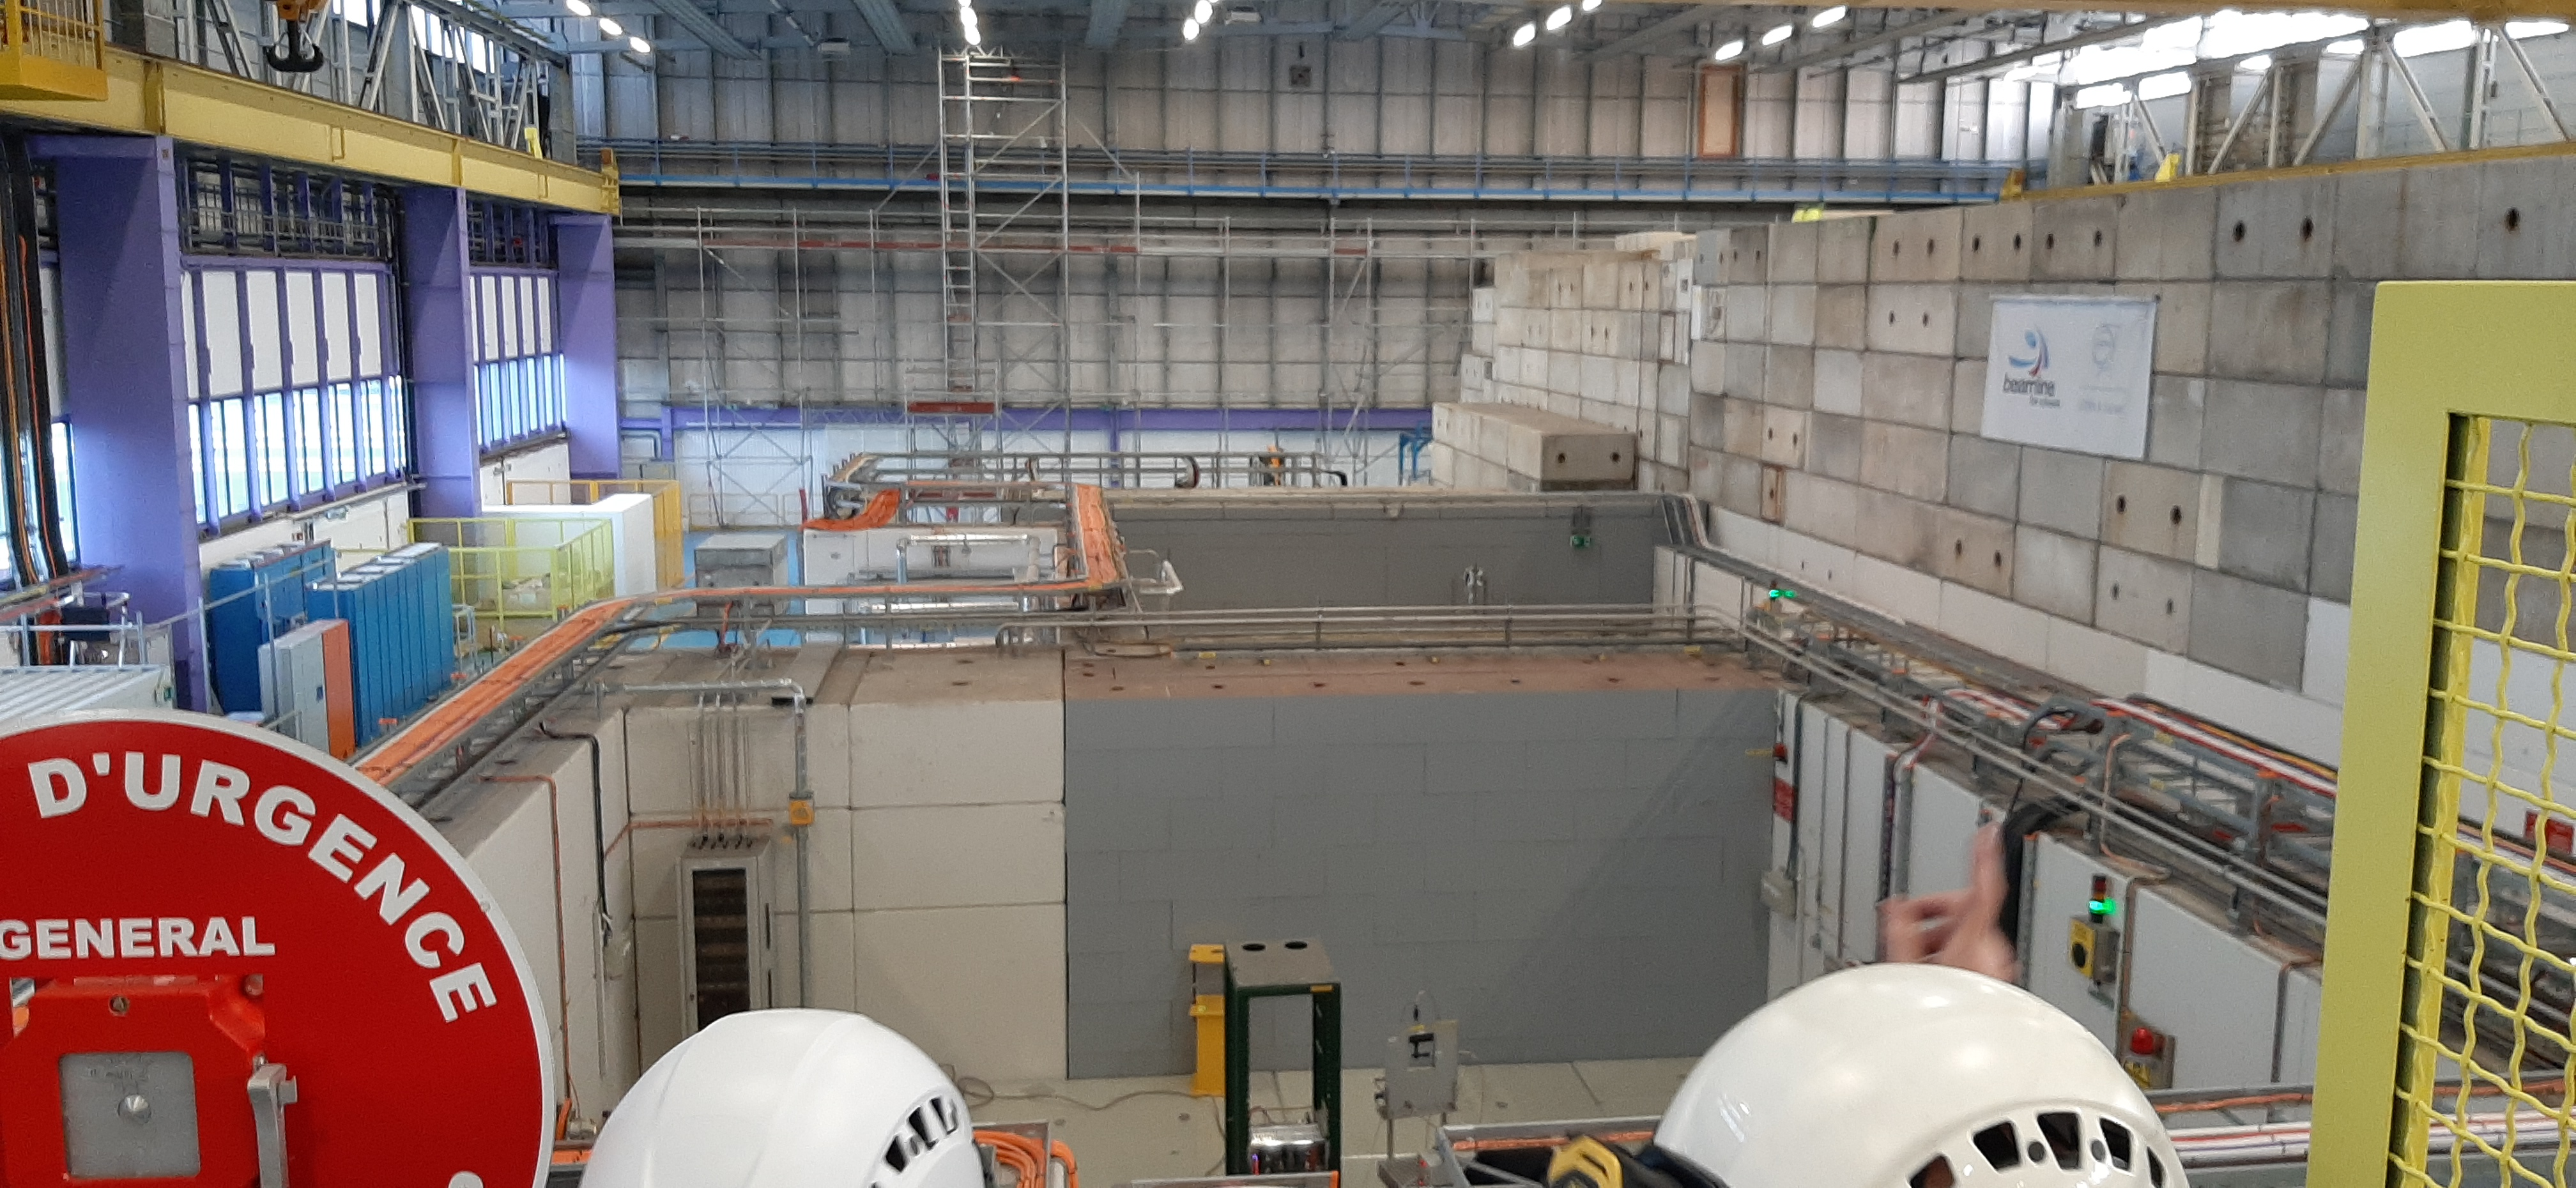
\includegraphics[width = 1.0\textwidth]{Plots/T9_BirdsView.jpg}
  \end{figure}
  \vspace{-0.2cm}
  \begin{center}
    \large East Area test beam hall
  \end{center}
\end{frame}

\begin{frame}{Start of test beam: Setup and preparations}
  \begin{figure}
    \centering
    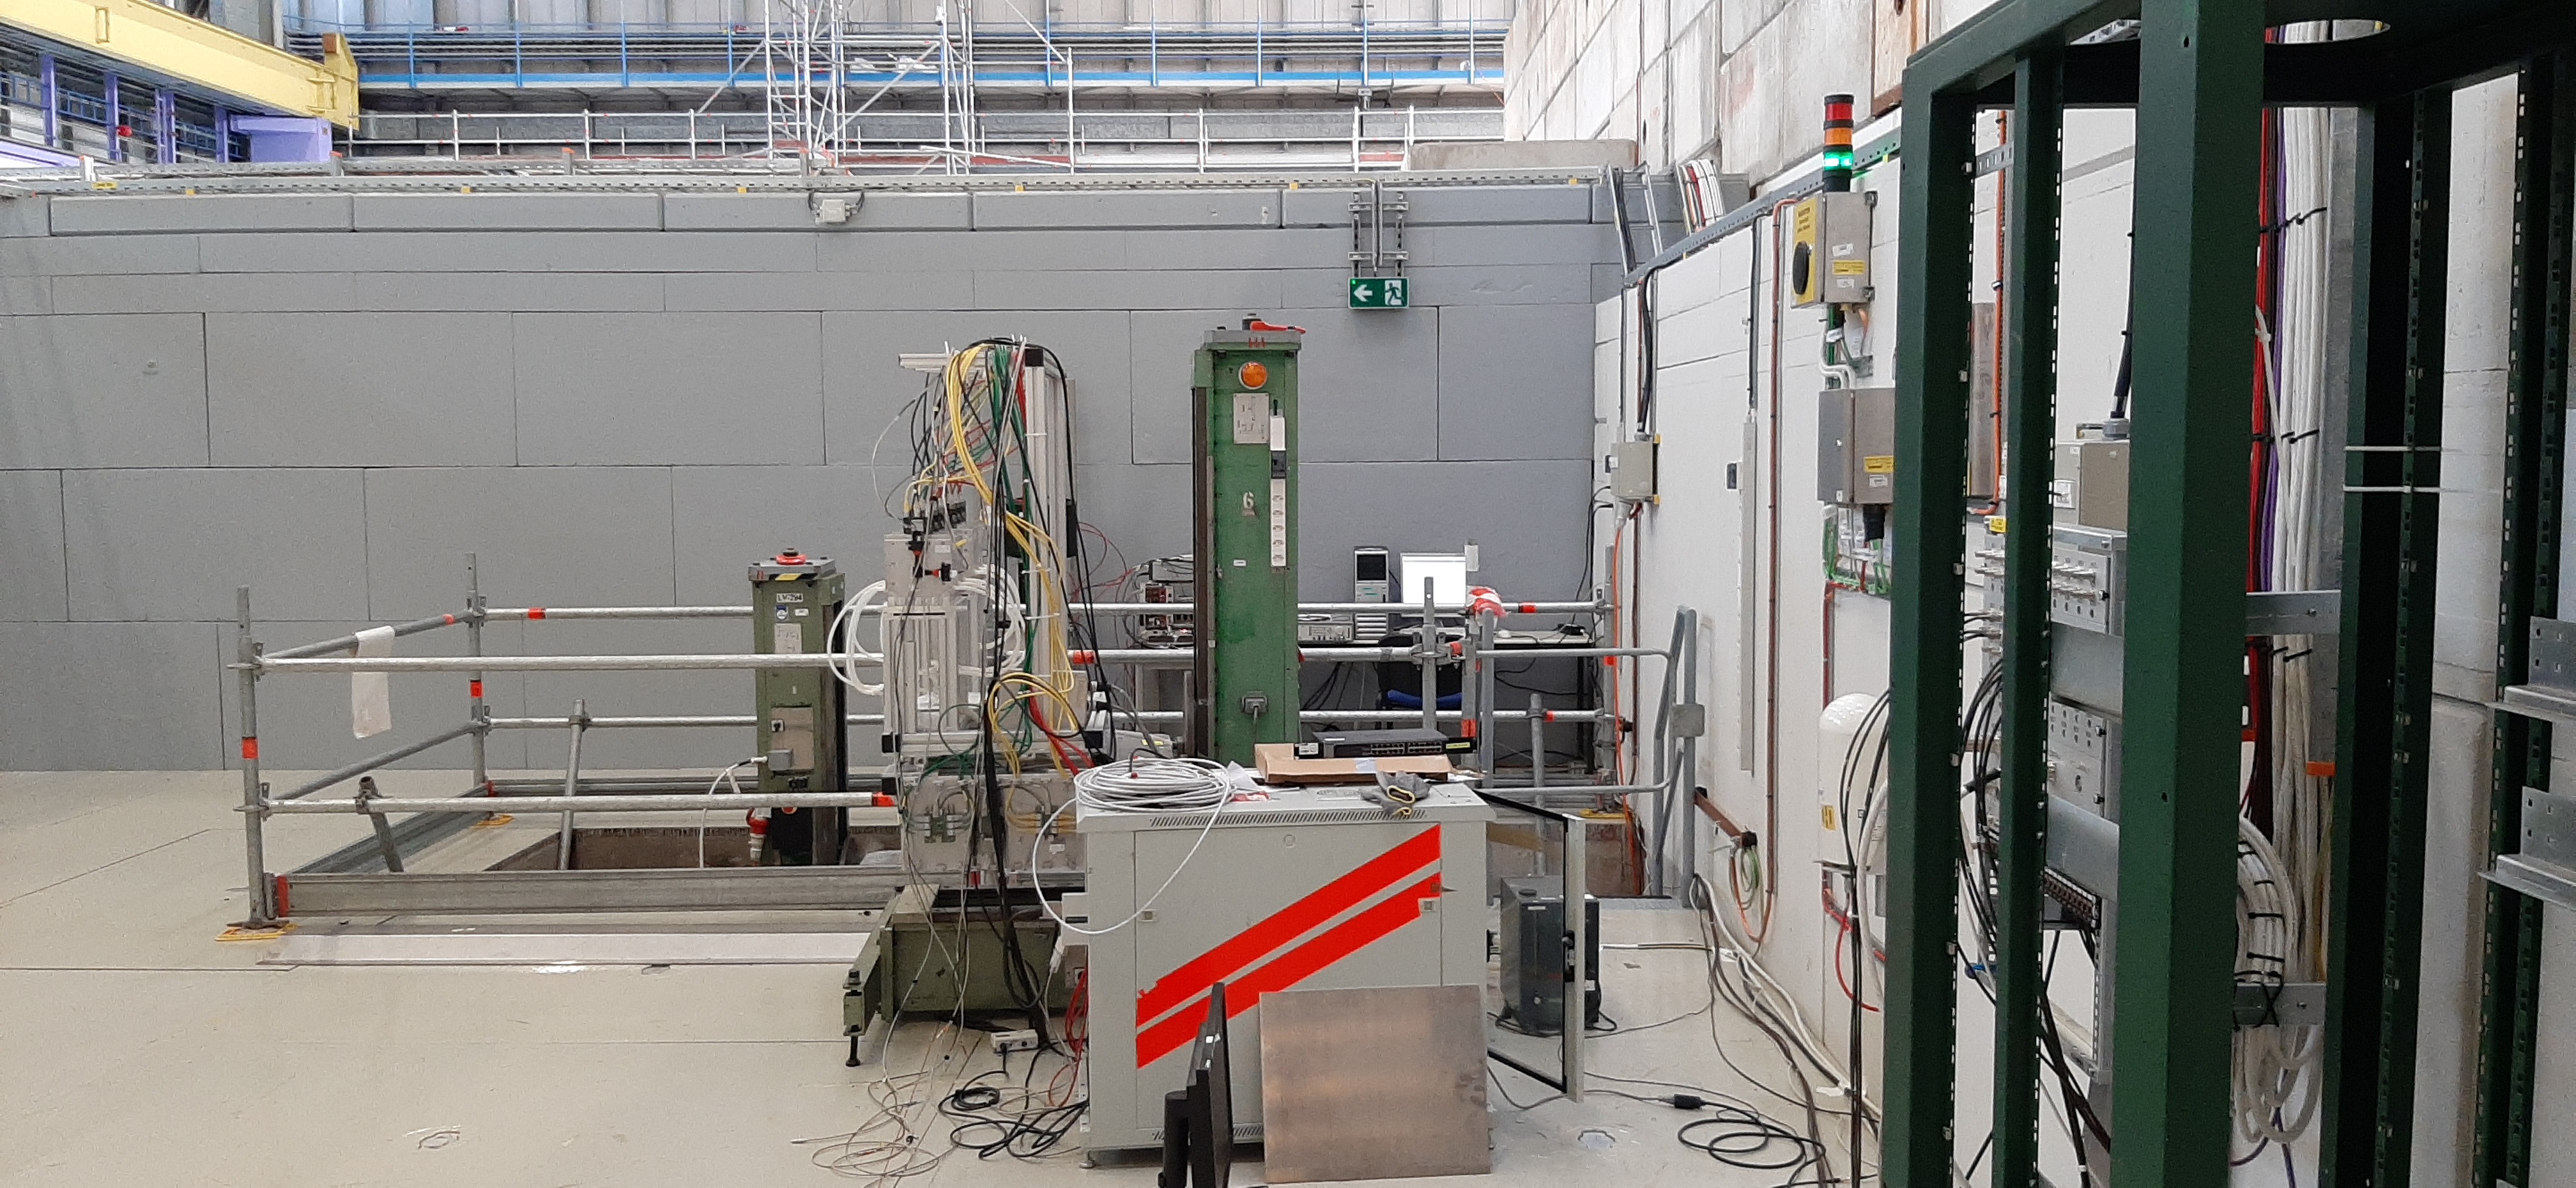
\includegraphics[width = 1.0\textwidth]{Plots/T9_Empty_floor.jpg}
  \end{figure}
  \vspace{-0.2cm}
  \begin{center}
    \large Background: Hole where concrete blocks were removed to fit TORCH\\
    \large Foreground: Beam telescope
  \end{center}
\end{frame}

\begin{frame}{Start of test beam: Setup and preparations}
  \begin{figure}
    \centering
    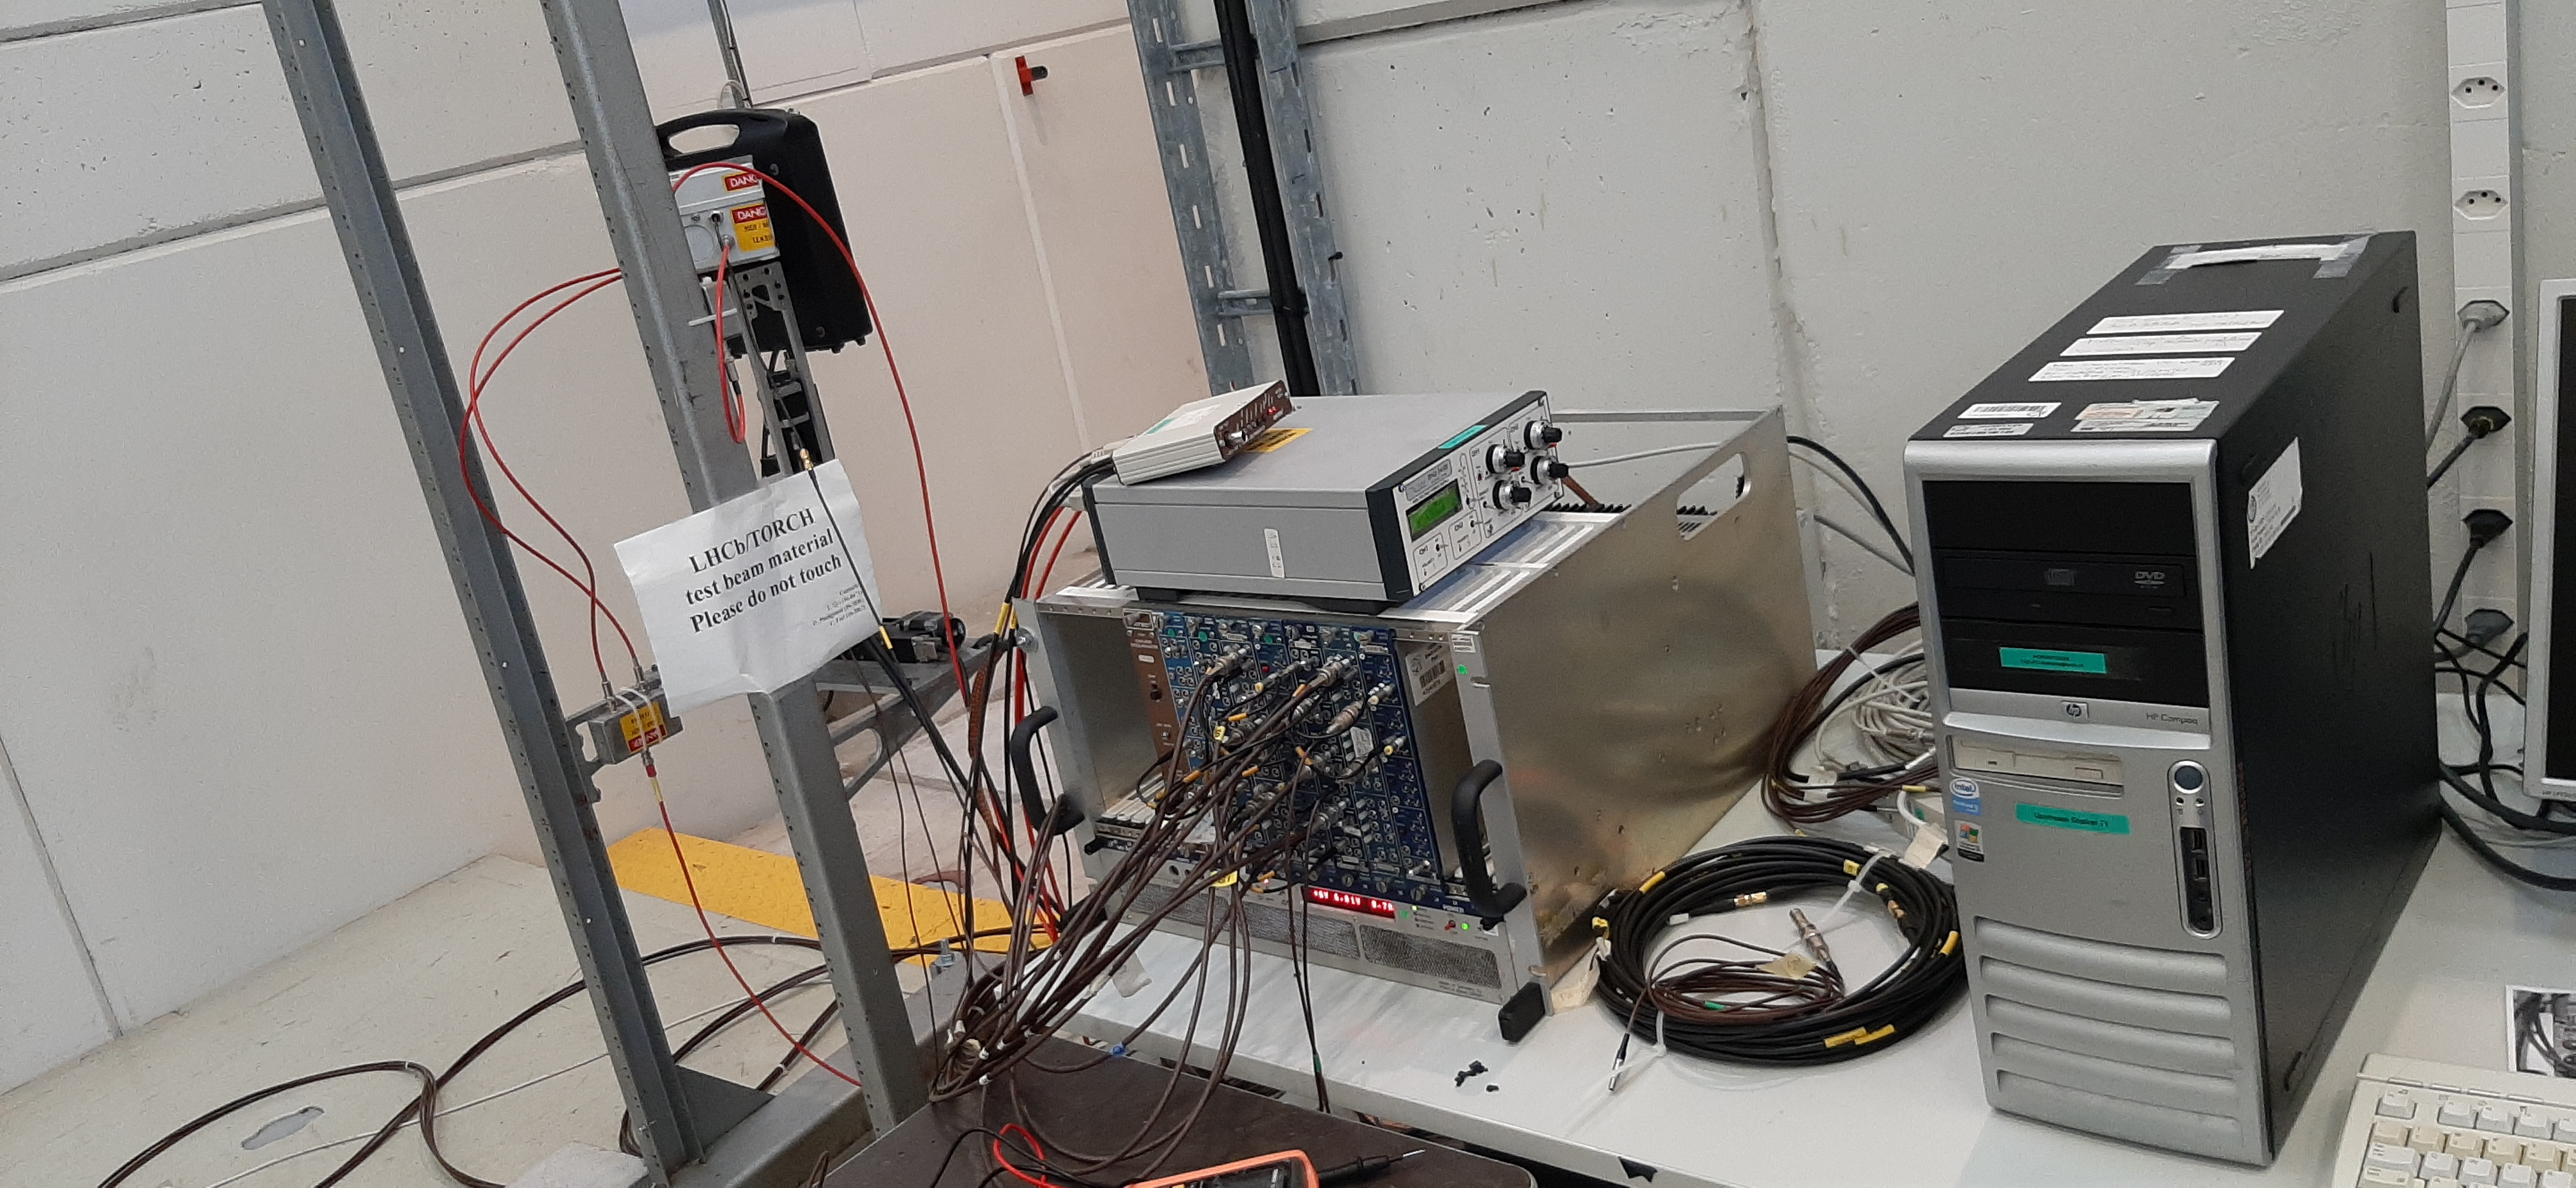
\includegraphics[width = 1.0\textwidth]{Plots/T1_overview.jpg}
  \end{figure}
  \vspace{-0.2cm}
  \begin{center}
    \large Final setup of T1 timing station, with F1 finger, two crossed scintillators, CFD (Const Fraction Discriminator) and NIM crate.
  \end{center}
\end{frame}

\begin{frame}{Start of test beam: Setup and preparations}
  \begin{figure}
    \centering
    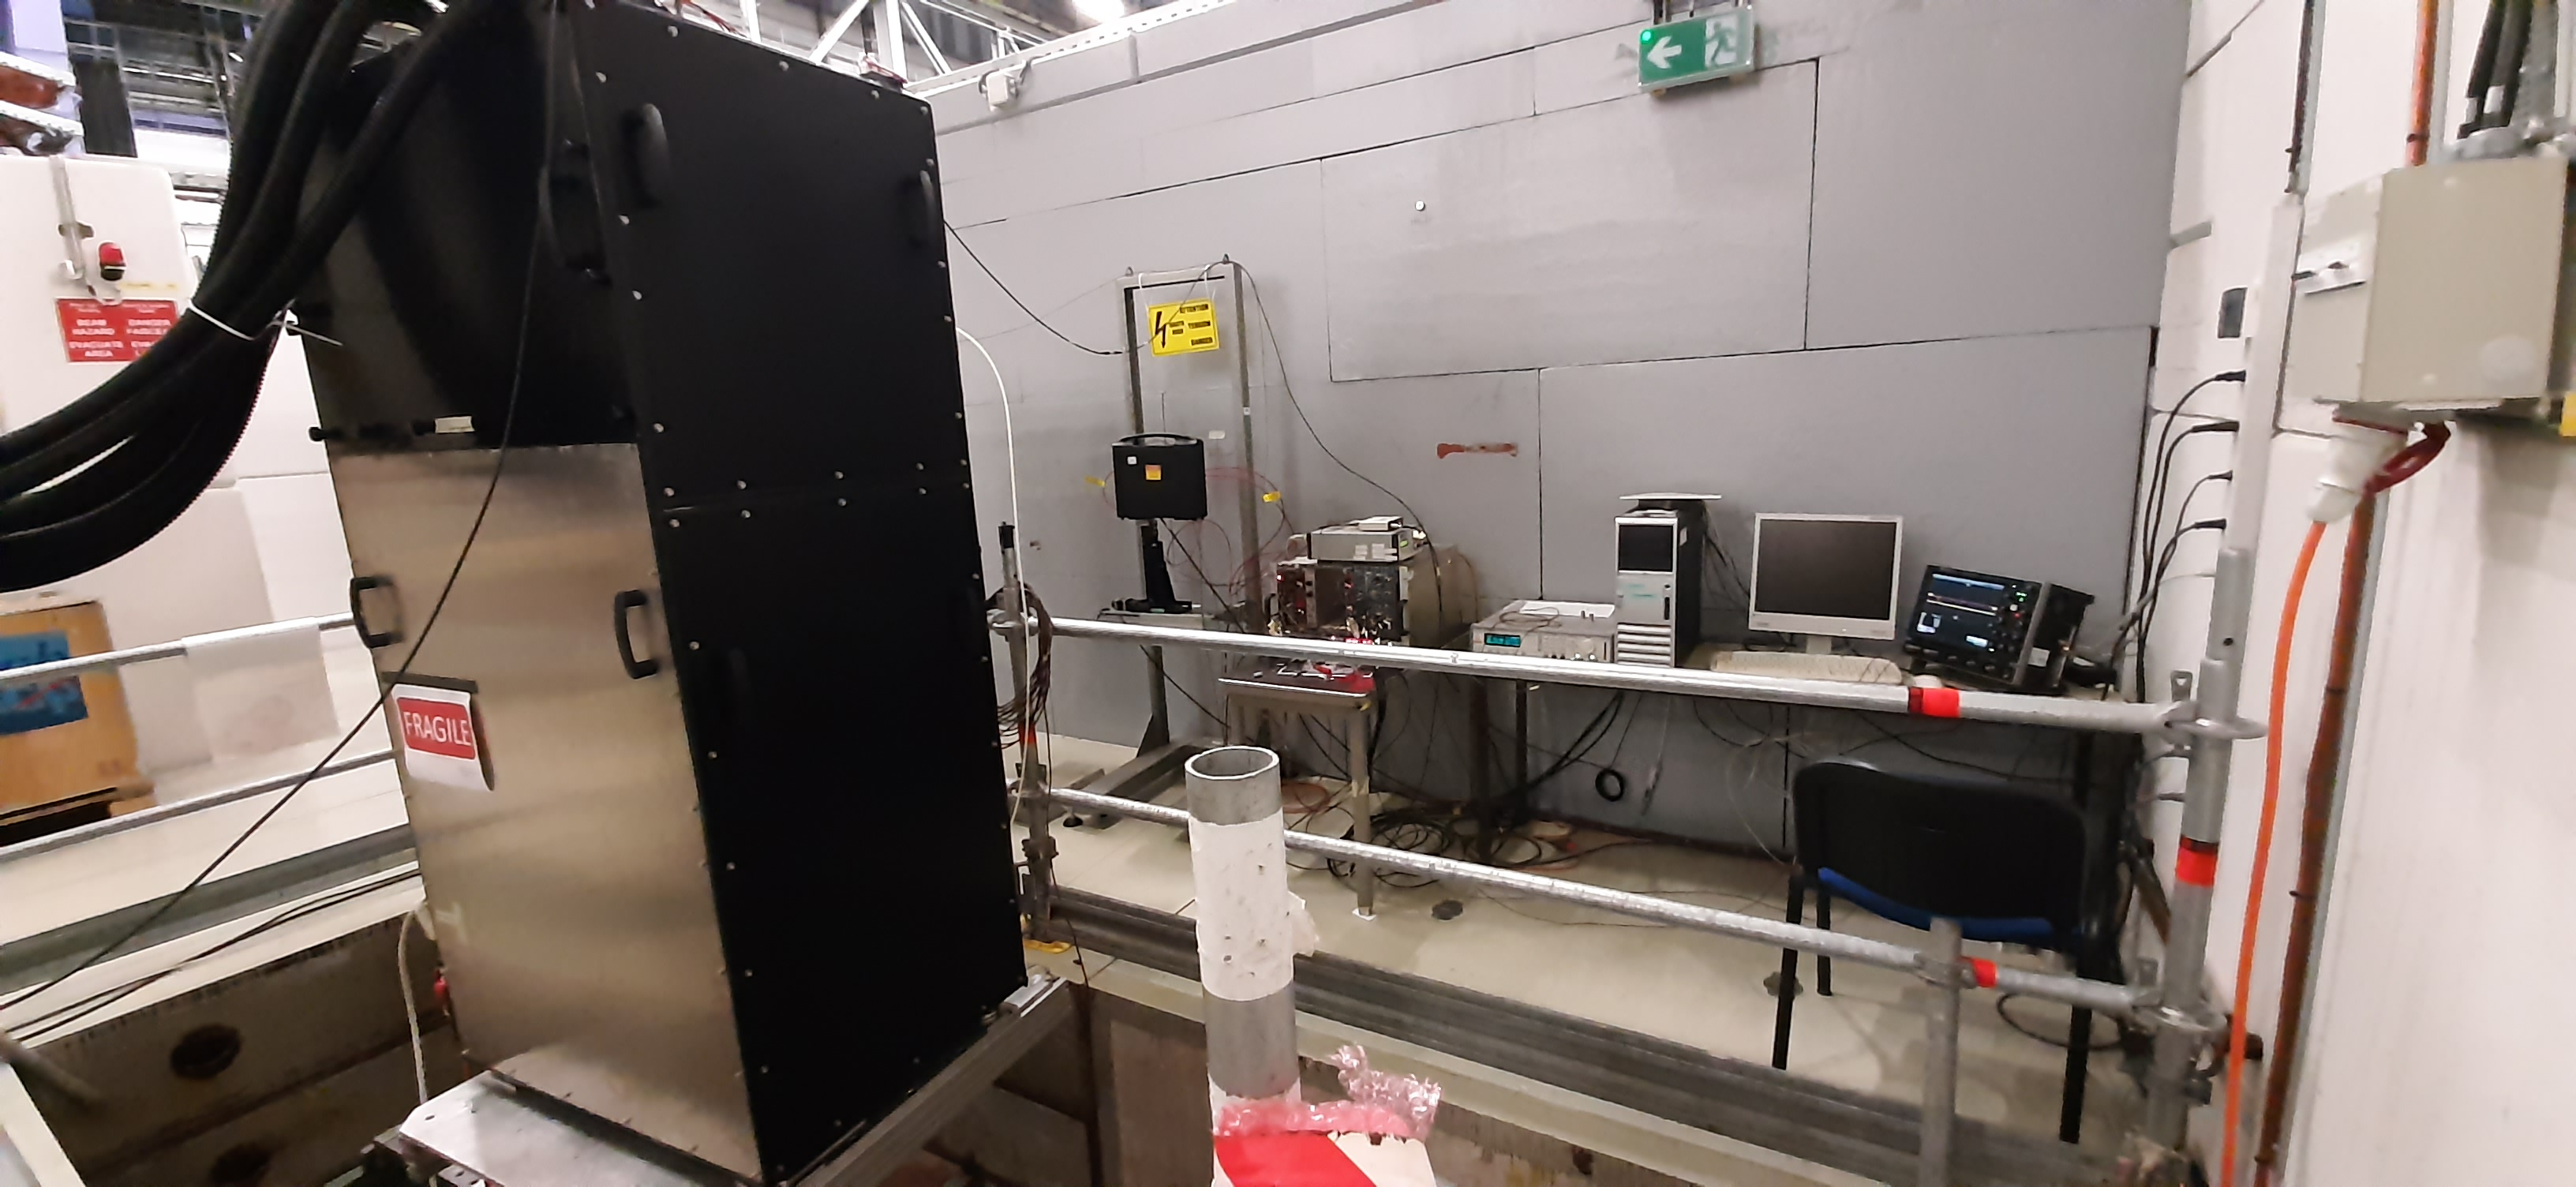
\includegraphics[width = 1.0\textwidth]{Plots/T2_overview.jpg}
  \end{figure}
  \vspace{-0.2cm}
  \begin{center}
    \large Final setup of T2 timing station, with F2 finger, two crossed scintillators, CFD (Const Fraction Discriminator) and NIM crate.
  \end{center}
\end{frame}

\begin{frame}{Start of test beam: Setup and preparations}
  \begin{figure}
    \centering
    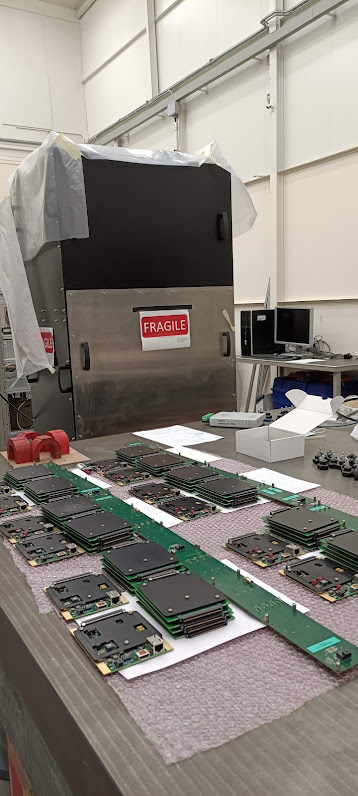
\includegraphics[width = 0.2\textwidth]{Plots/Electronics_1.jpg}
    \hspace{1cm}
    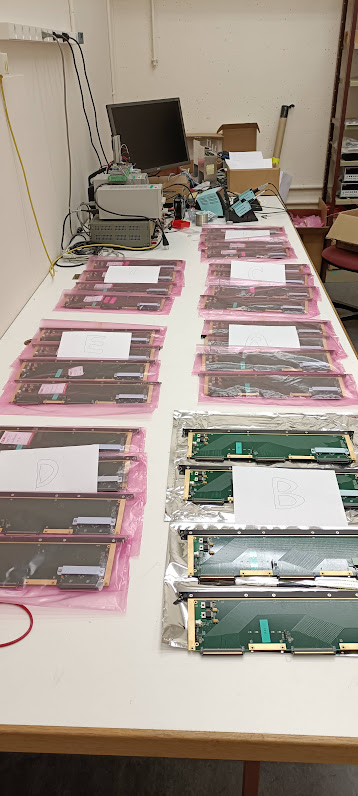
\includegraphics[width = 0.2\textwidth]{Plots/Electronics_2.jpg}
  \end{figure}
  \vspace{-0.2cm}
  \begin{center}
    \large Meanwhile, in the lab, the electronics is prepared carefully...
  \end{center}
\end{frame}

\begin{frame}{Start of test beam: Setup and preparations}
  \begin{figure}
    \centering
    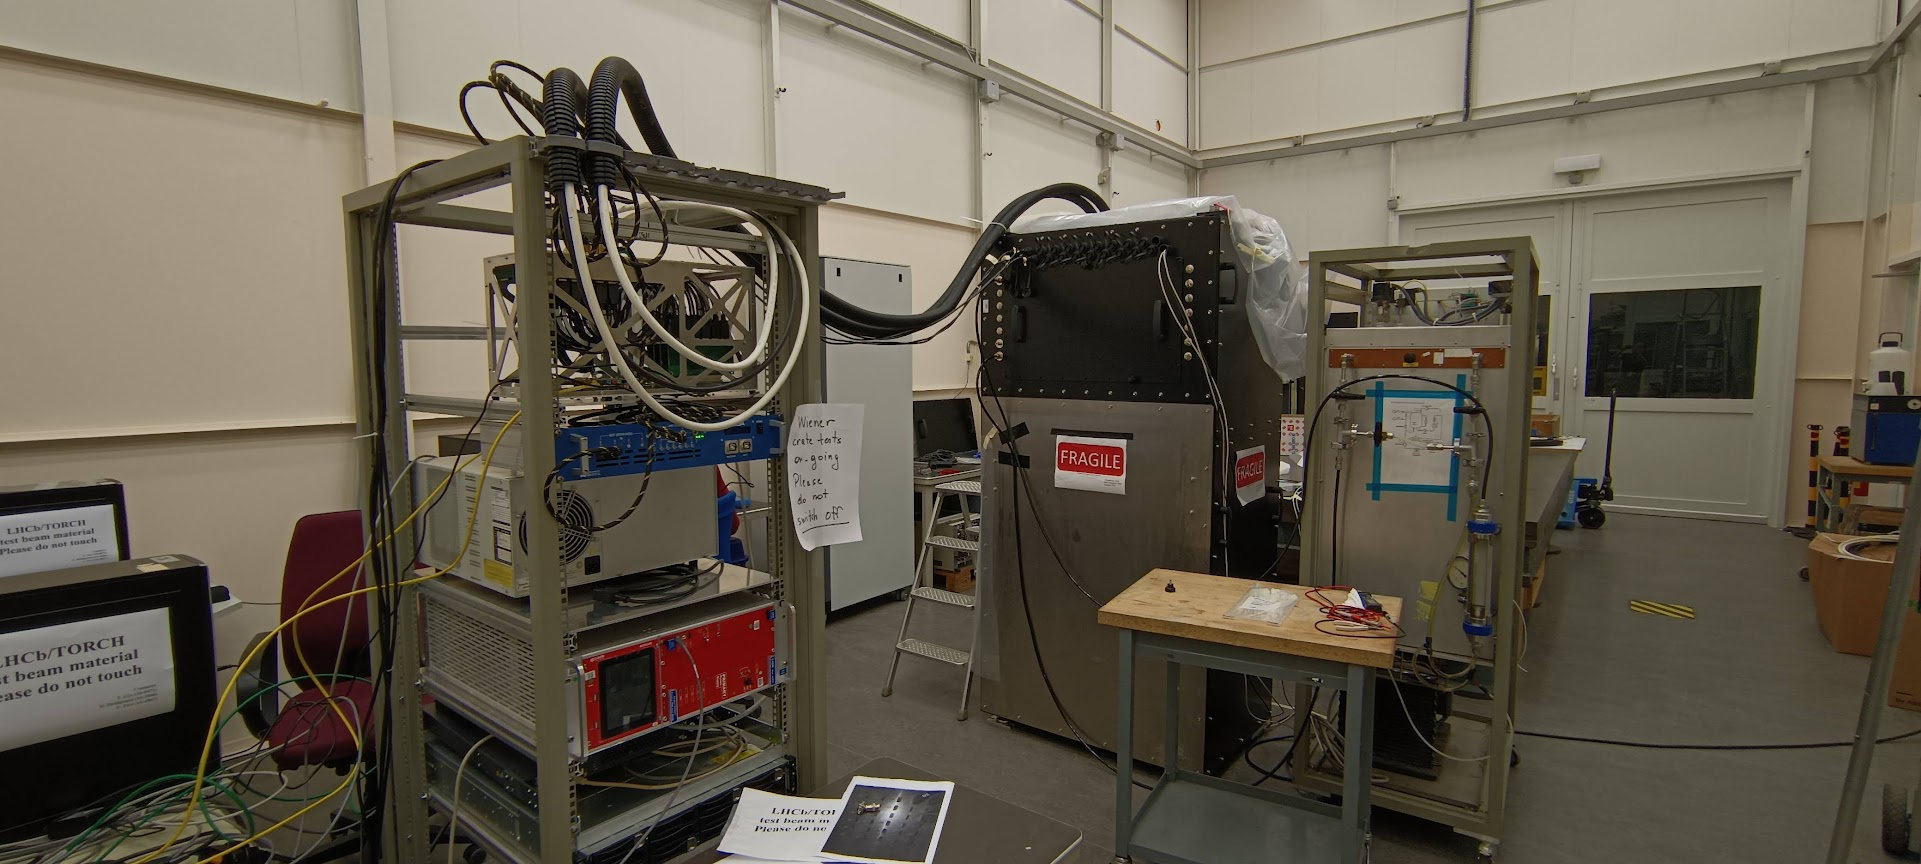
\includegraphics[width = 1.0\textwidth]{Plots/TORCH_lab.jpg}
  \end{figure}
  \vspace{-0.2cm}
  \begin{center}
    \large ... and the MCPs are safely installed and cabled inside proto-TORCH
  \end{center}
\end{frame}

\begin{frame}{Start of test beam: Setup and preparations}
  \begin{figure}
    \centering
    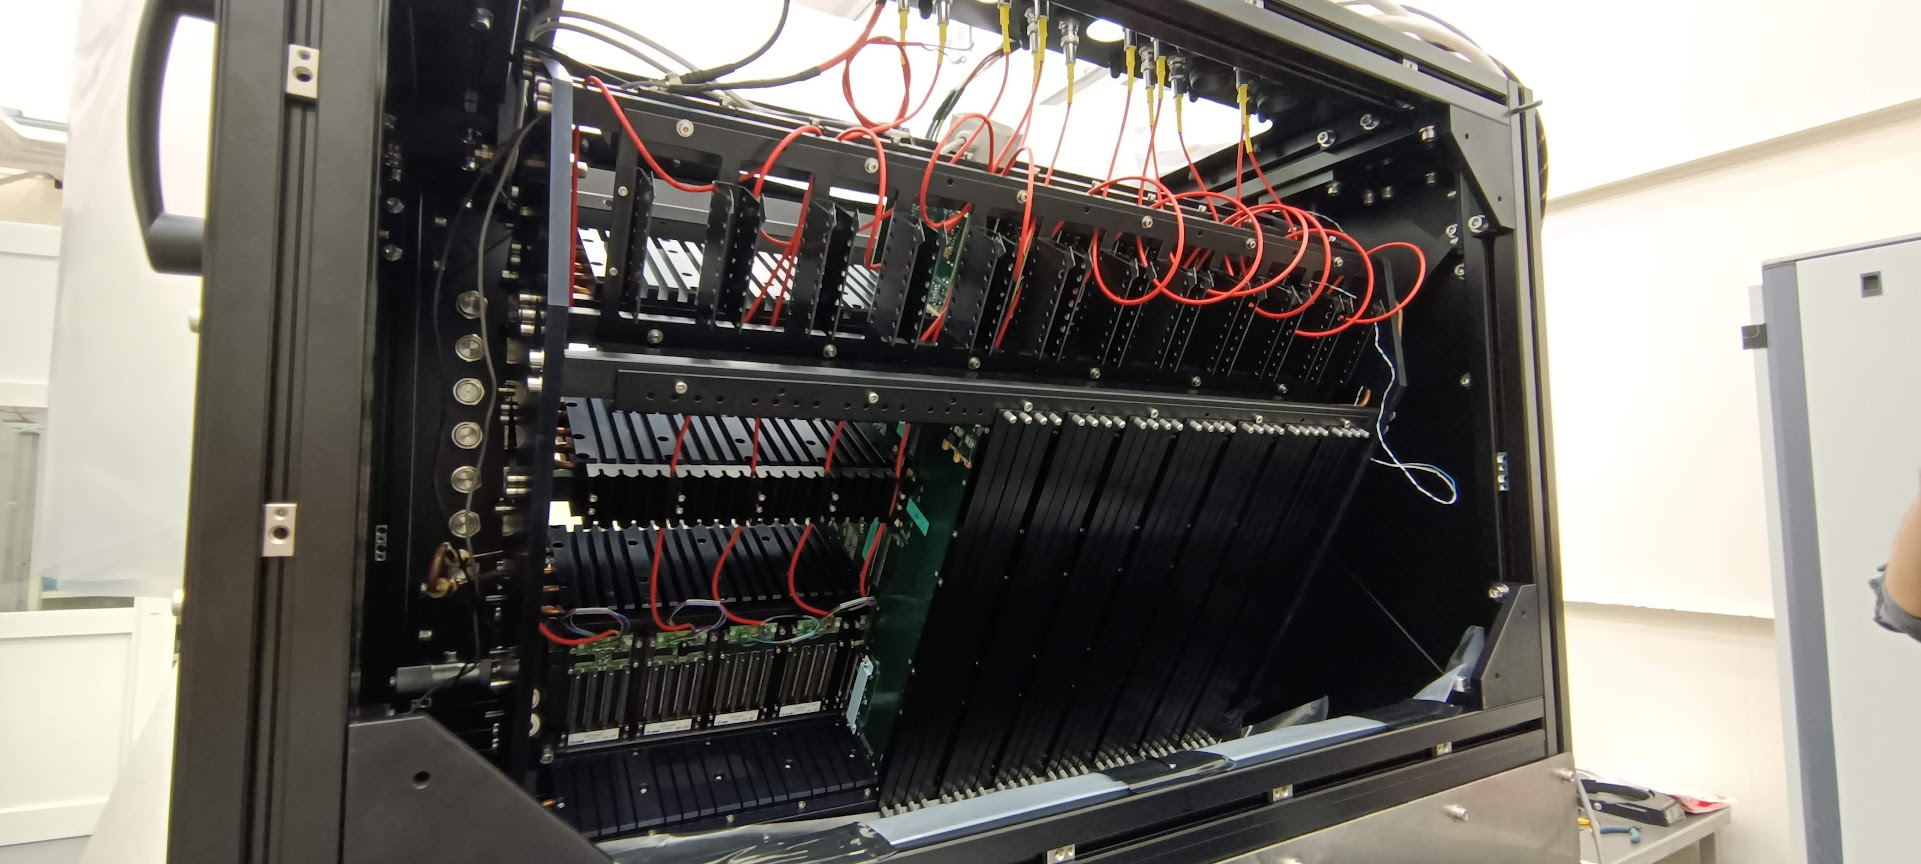
\includegraphics[width = 1.0\textwidth]{Plots/MCP_installation.jpg}
  \end{figure}
  \vspace{-0.2cm}
  \begin{center}
    \large 11 MCPs are installed in total, 7 MCPs have readout electronics
  \end{center}
\end{frame}

\section{Get ready to turn everything on: Will it work?}
\begin{frame}{Get ready to turn everything on: Will it work?}
  \begin{itemize}
    \item{Week 2: TORCH enters T9}
    \begin{itemize}
      \item{Transport of Proto-TORCH from lab to T9}
      \item{Lots of cabling}
      \item{Safety inspection}
    \end{itemize}
  \end{itemize}
  \begin{figure}
    \centering
    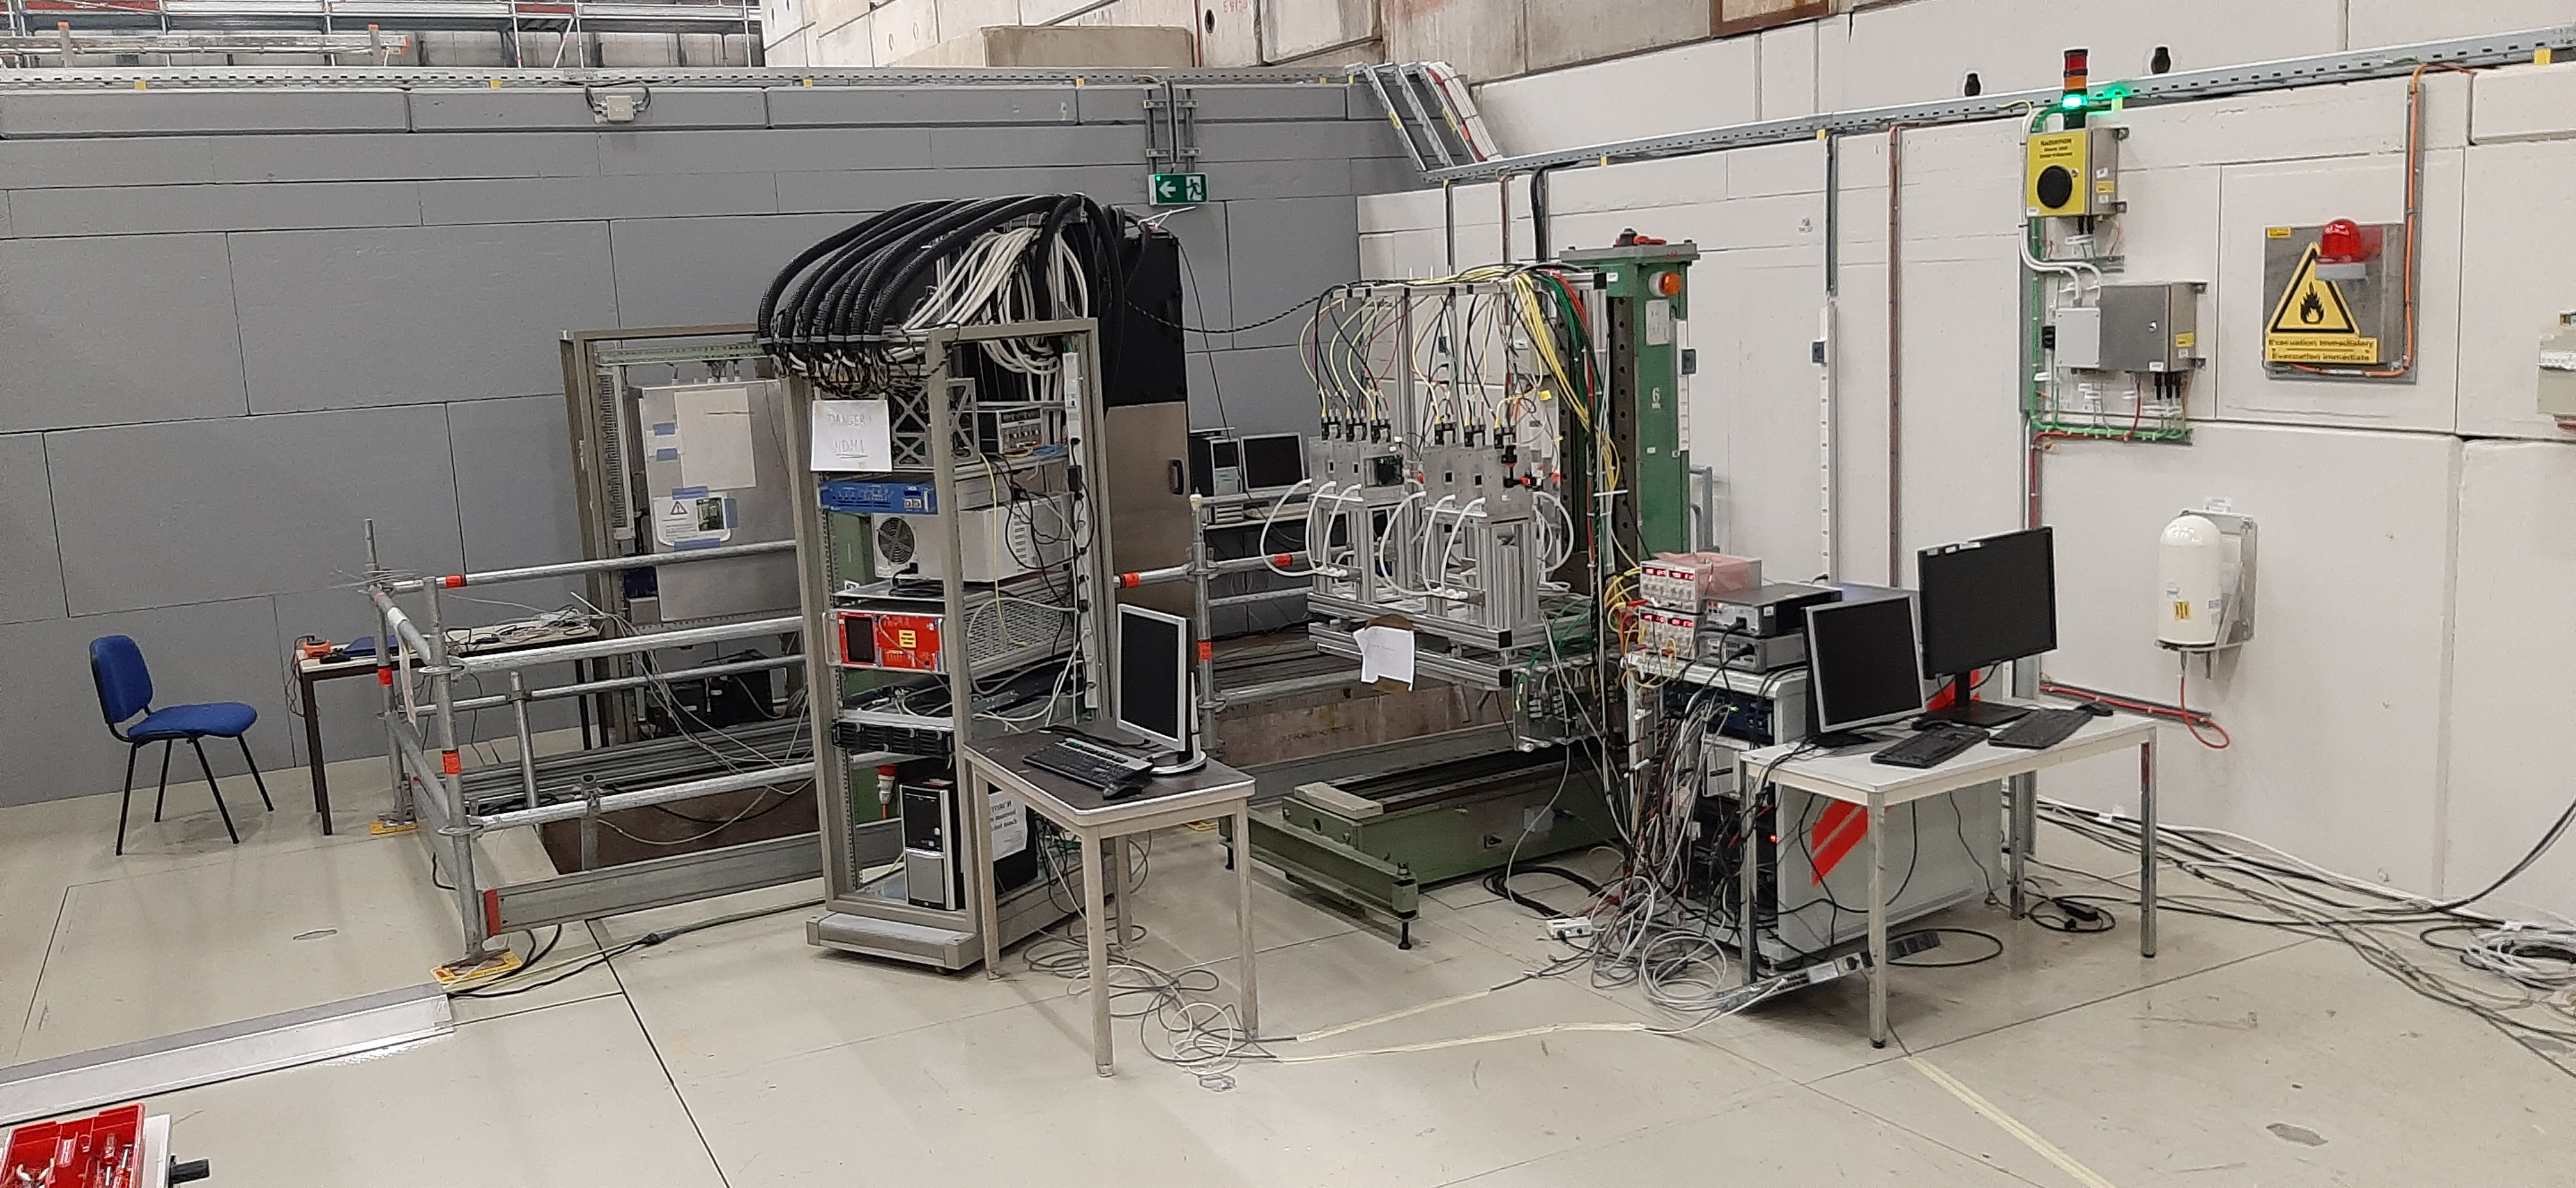
\includegraphics[width = 0.8\textwidth]{Plots/TelescopeTORCHoverview.jpg}
  \end{figure}
  \begin{center}
    \large Lesson from safety inspection: HDMI cables are dangerous!
  \end{center}
\end{frame}

\begin{frame}{Get ready to turn everything on: Will it work?}
  \begin{figure}
    \centering
    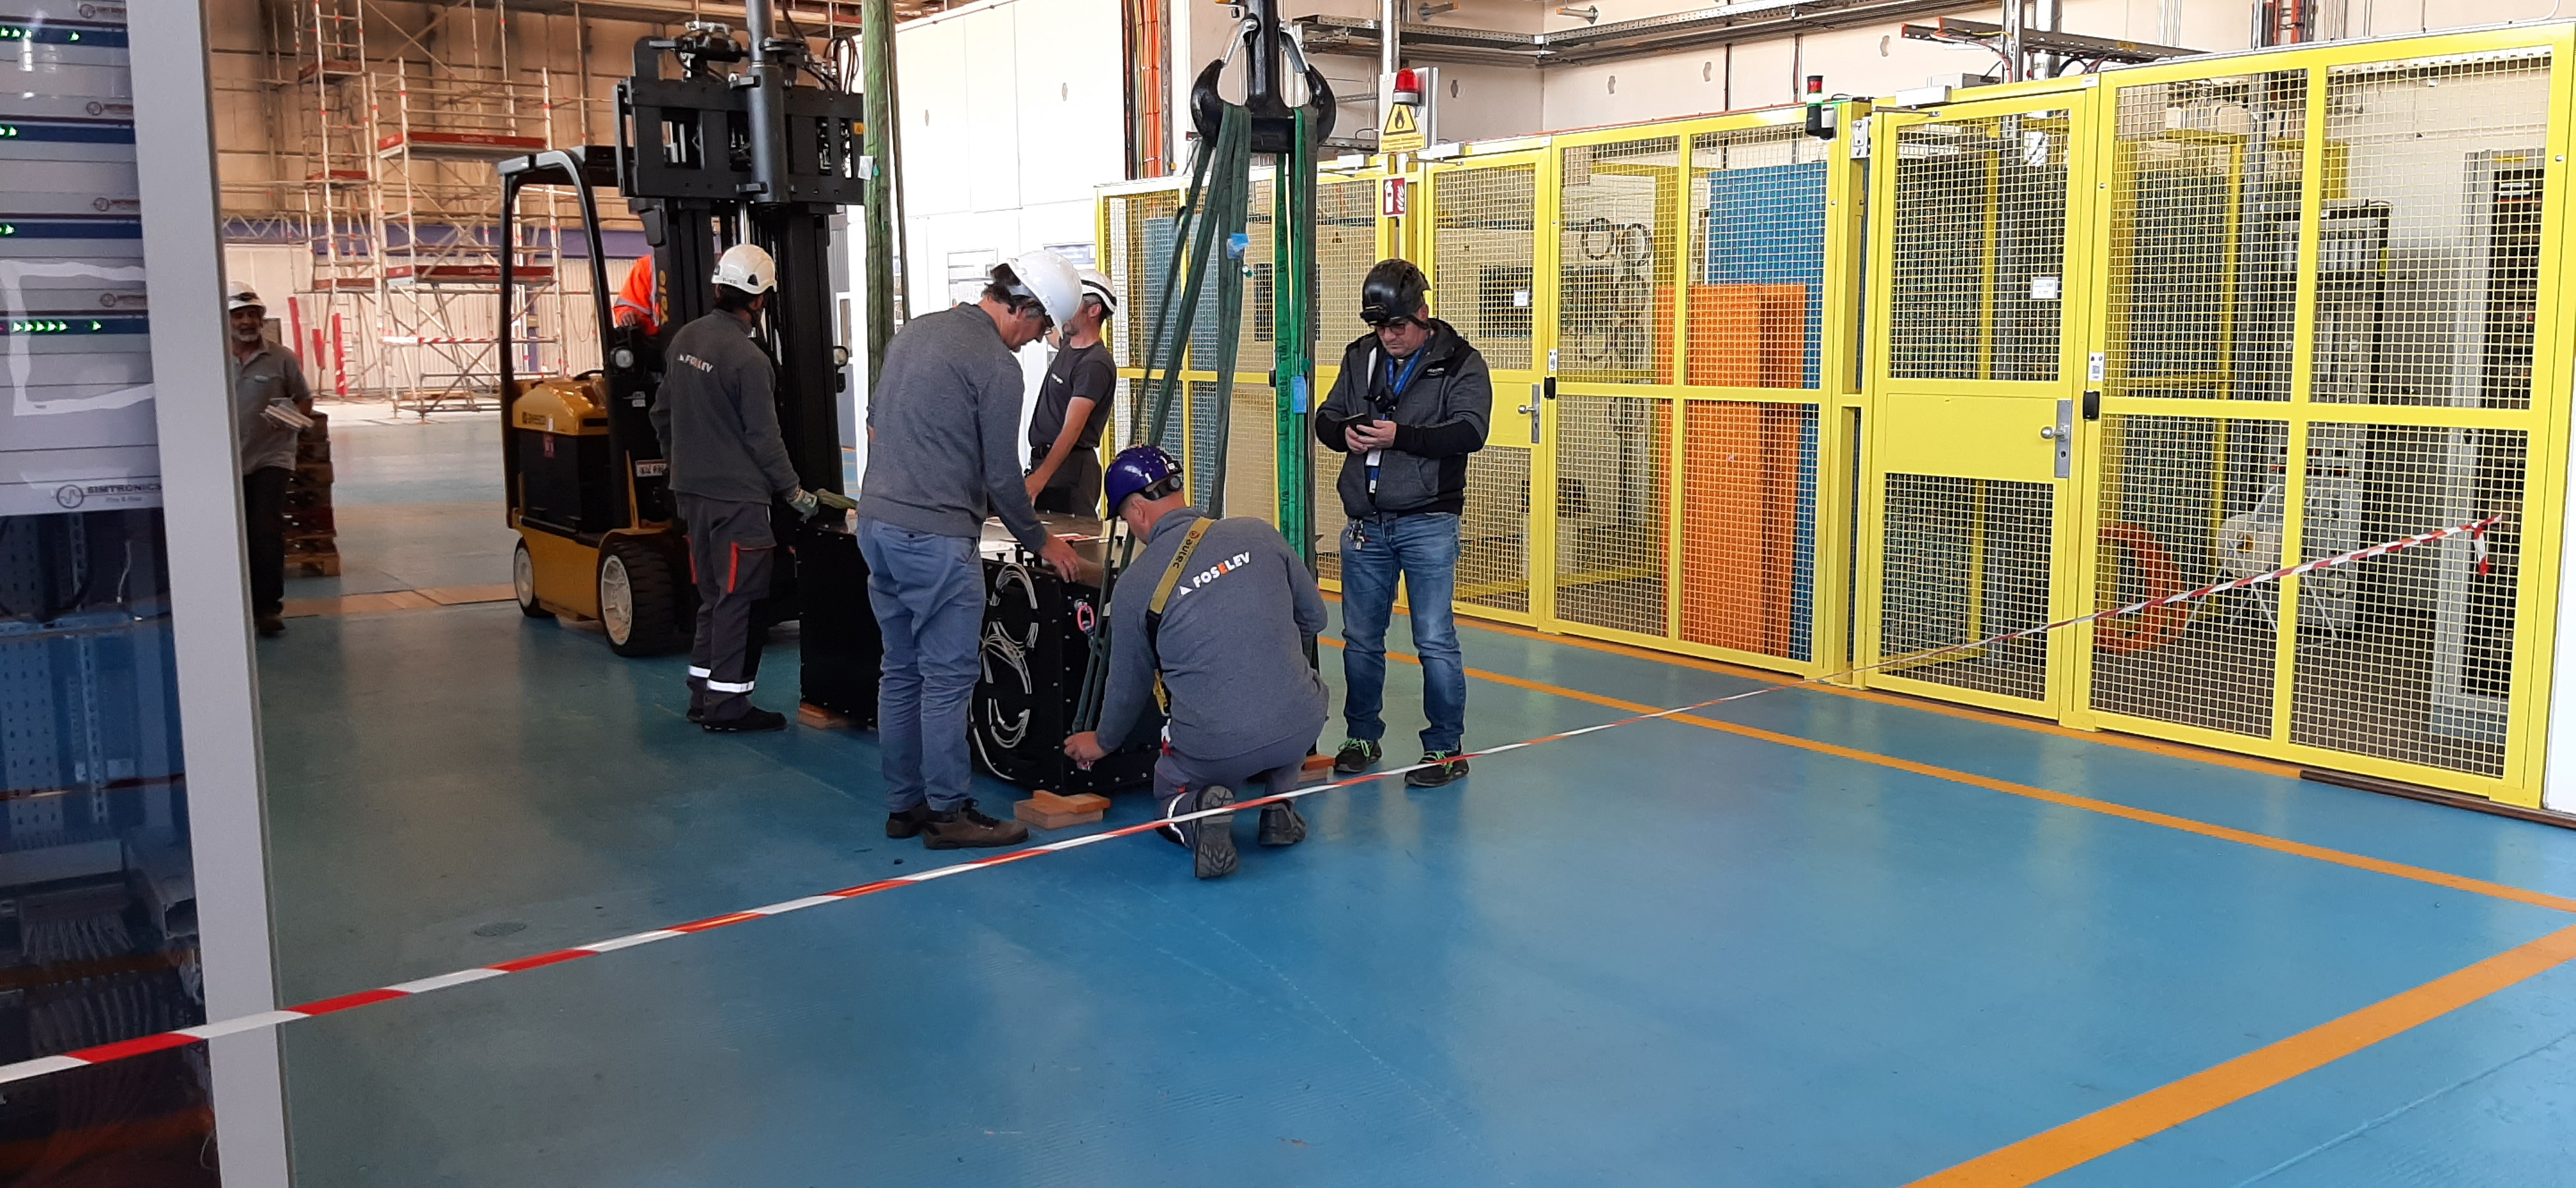
\includegraphics[width = 0.45\textwidth]{Plots/TORCH_transport_0.jpg}
    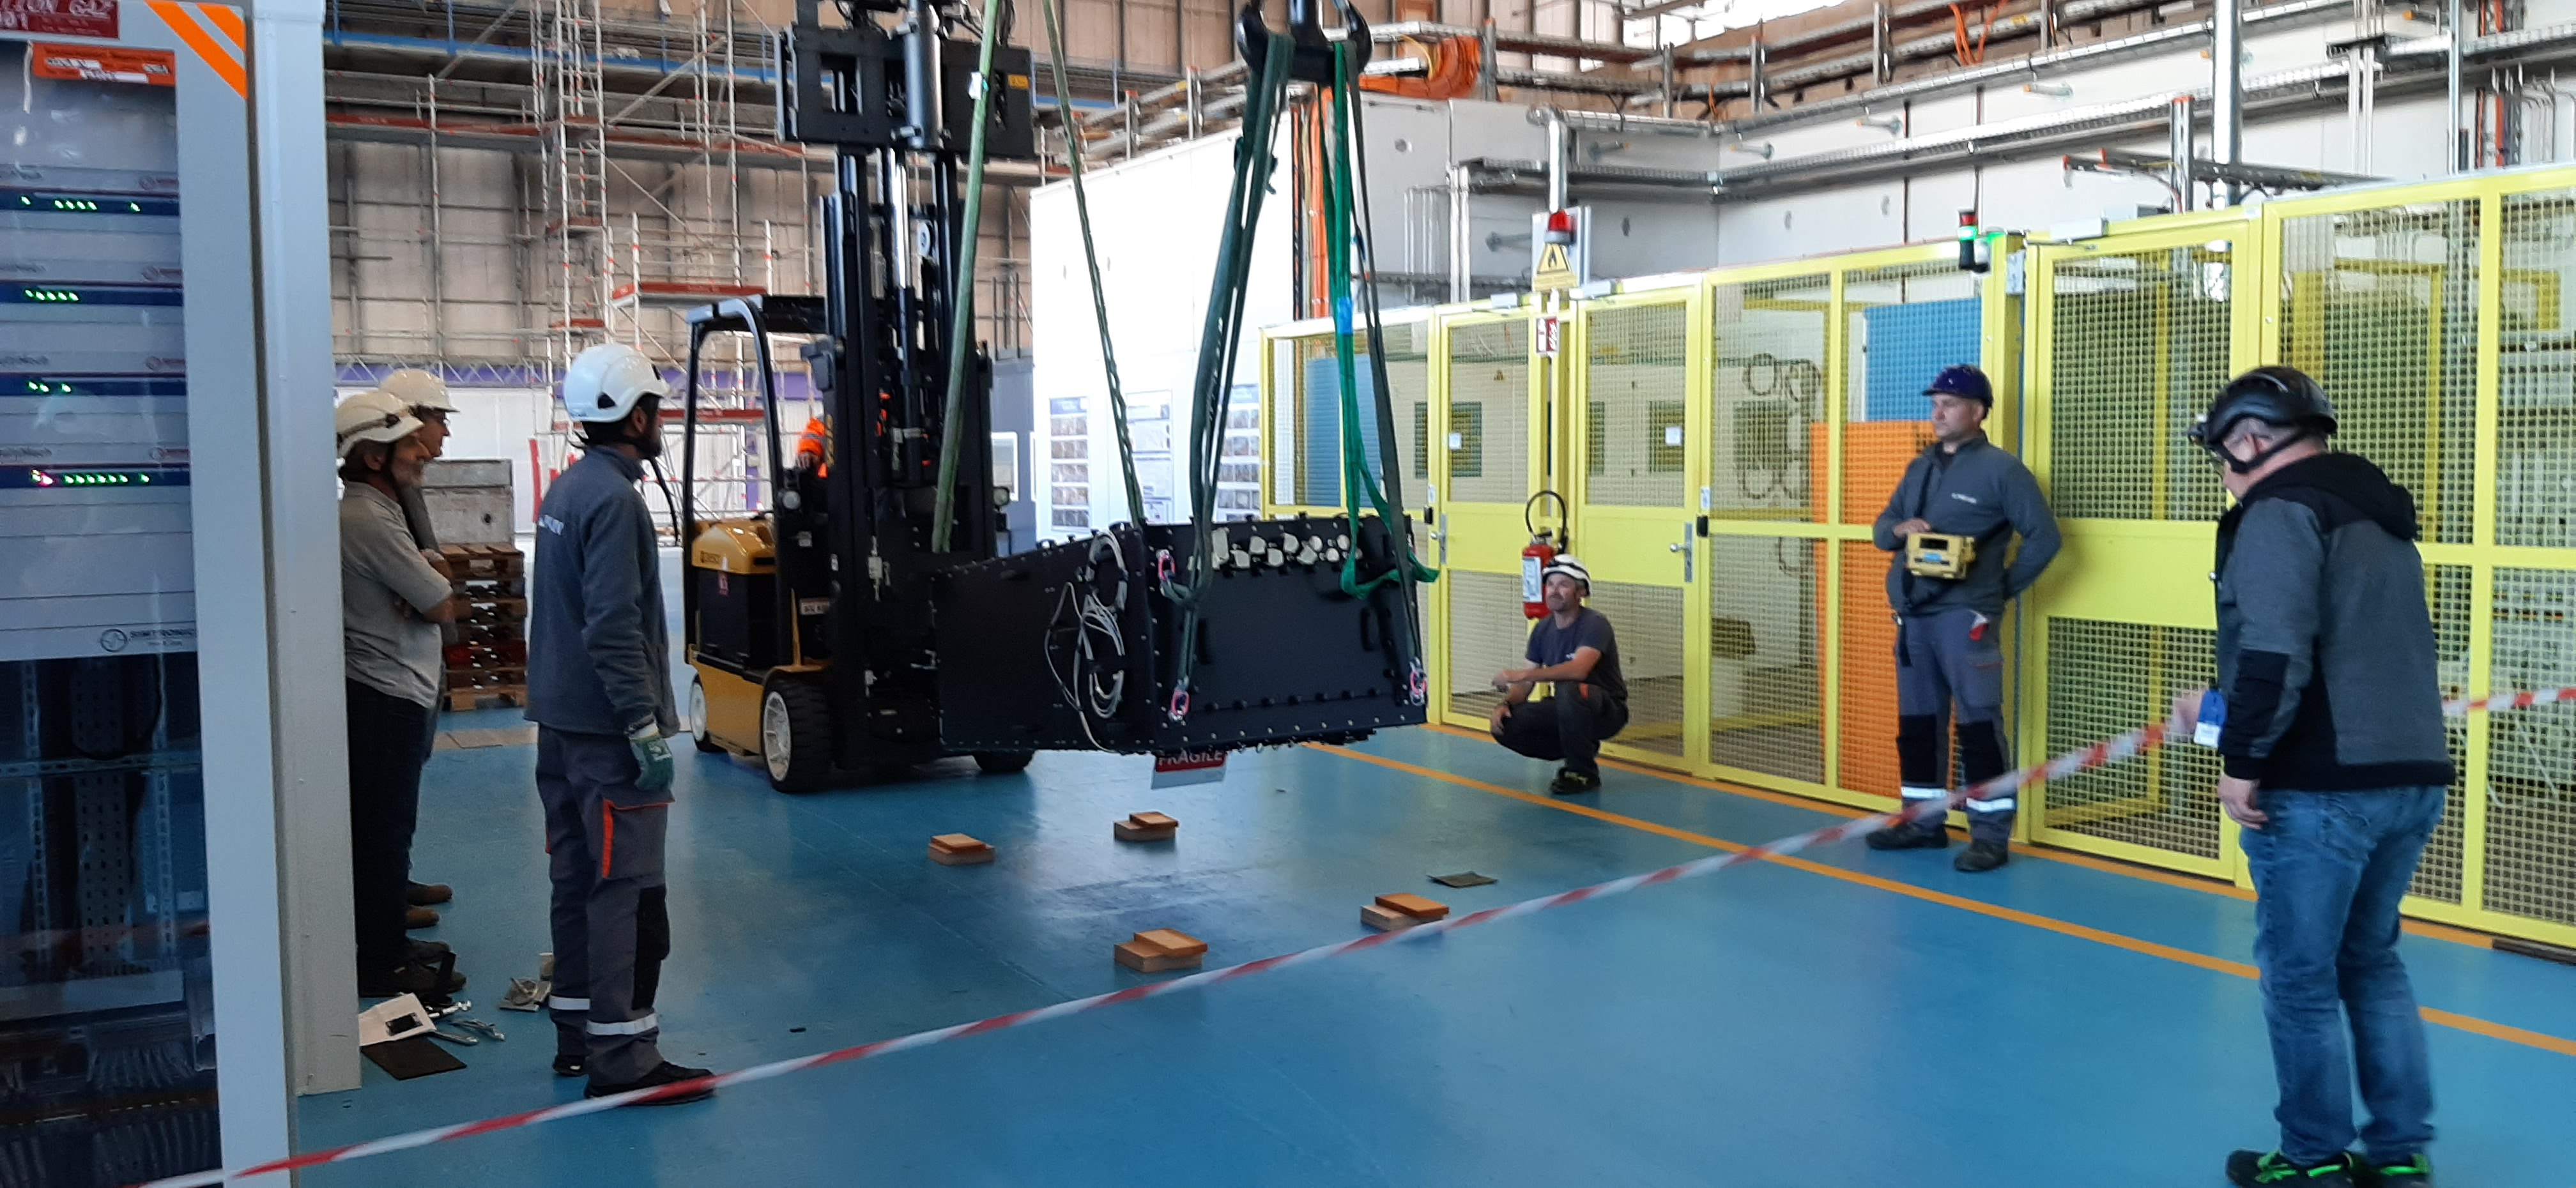
\includegraphics[width = 0.45\textwidth]{Plots/TORCH_transport_1.jpg}
    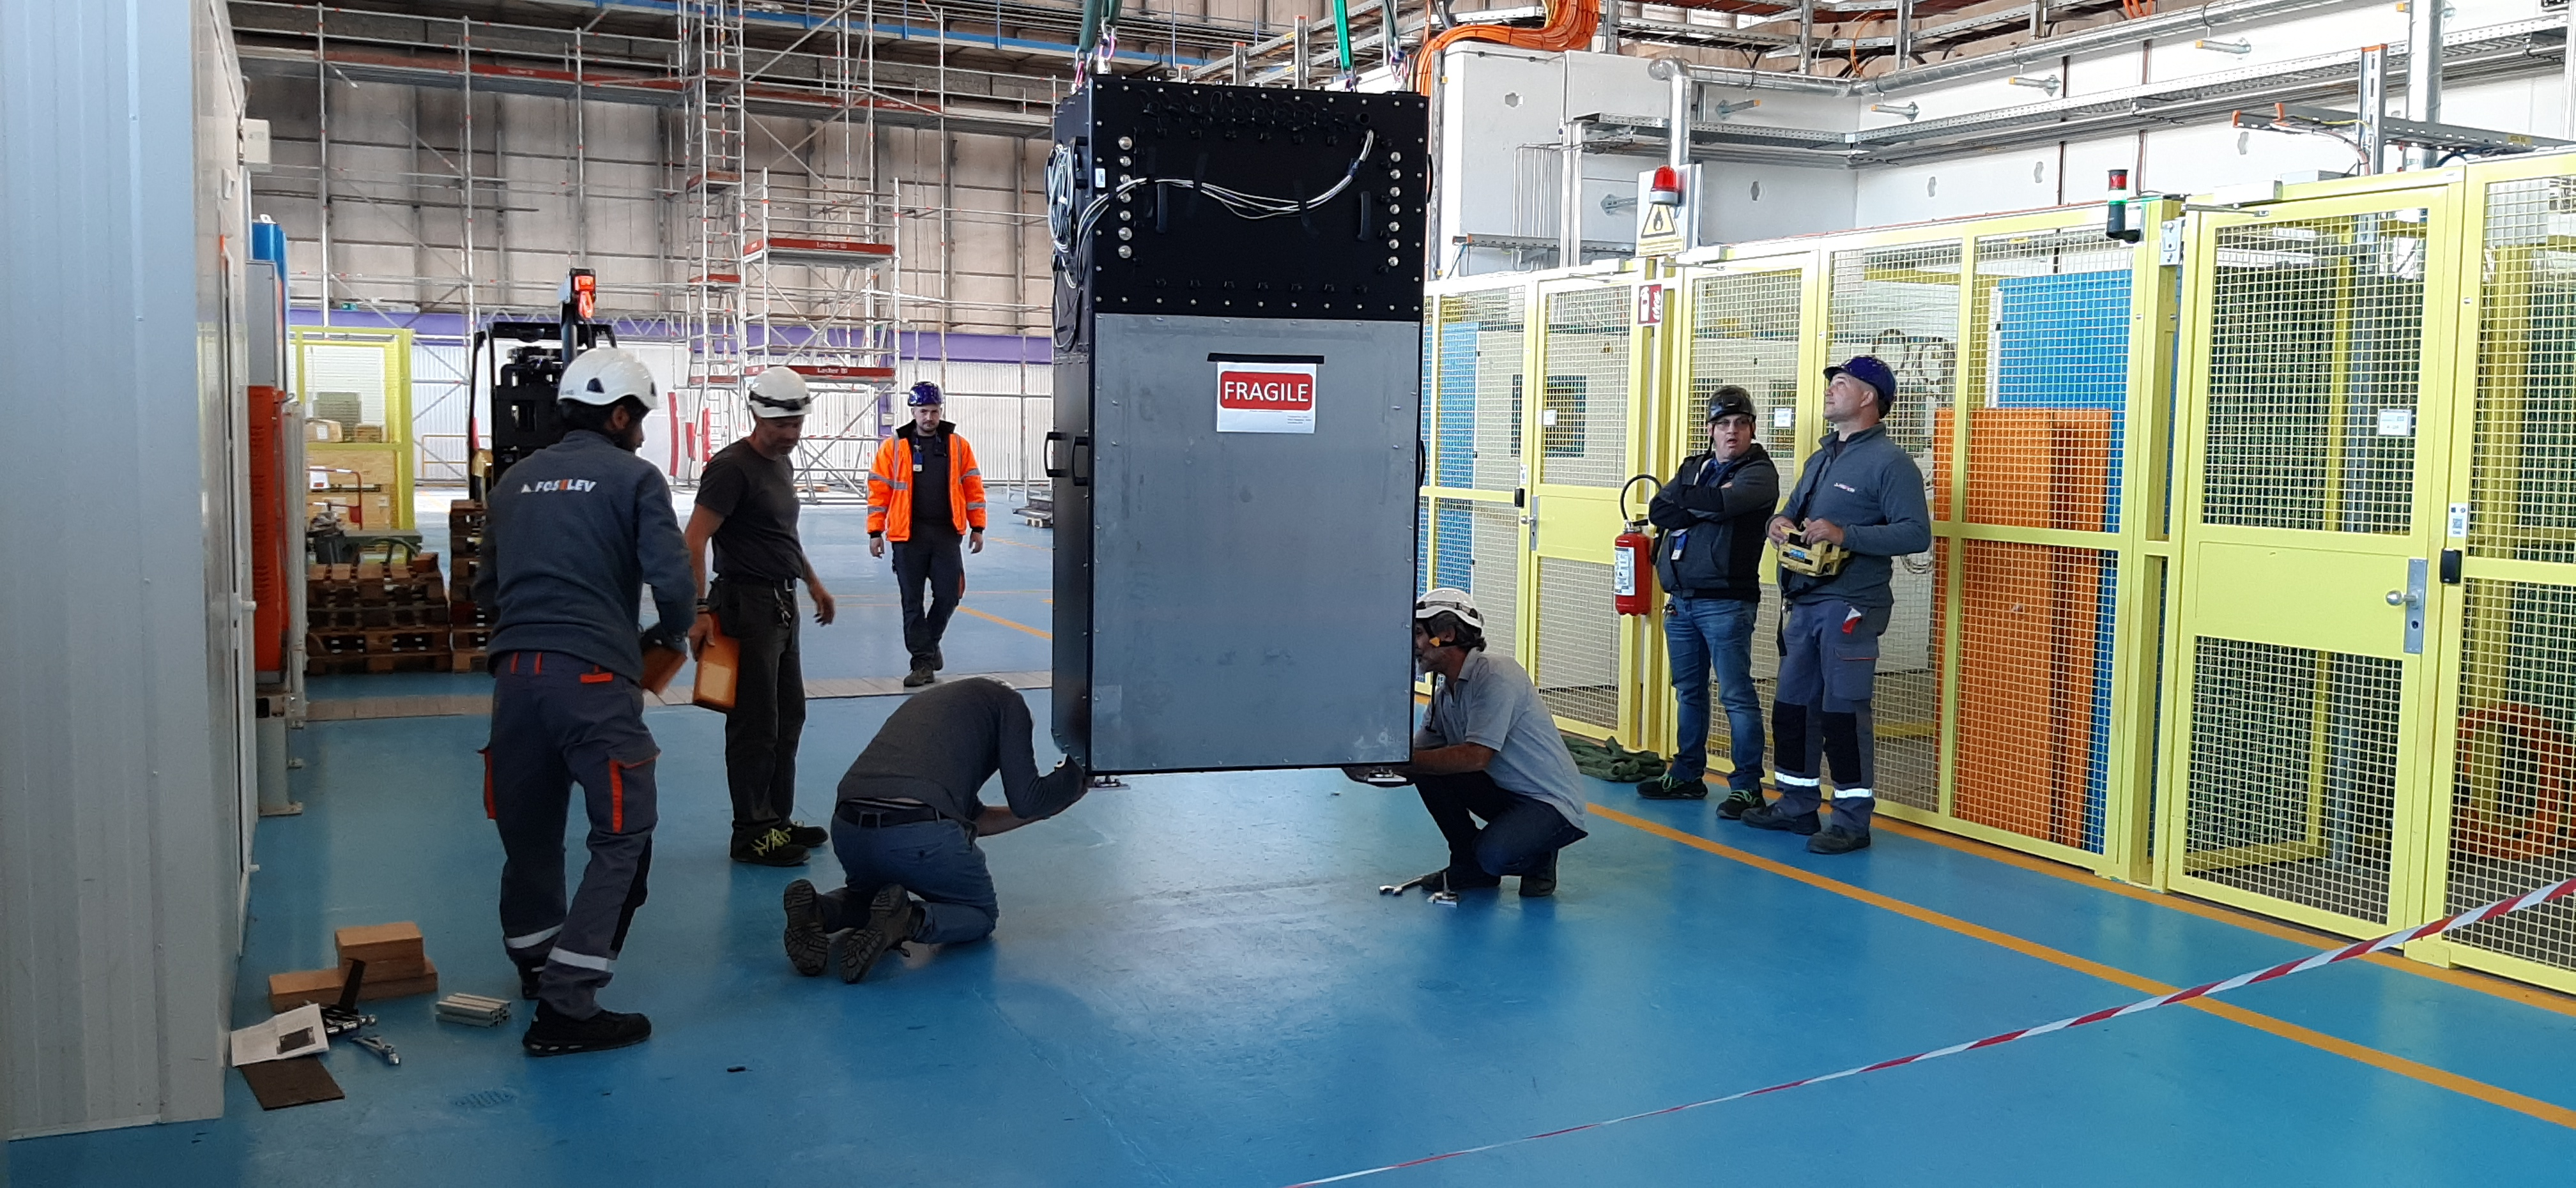
\includegraphics[width = 0.45\textwidth]{Plots/TORCH_transport_2.jpg}
    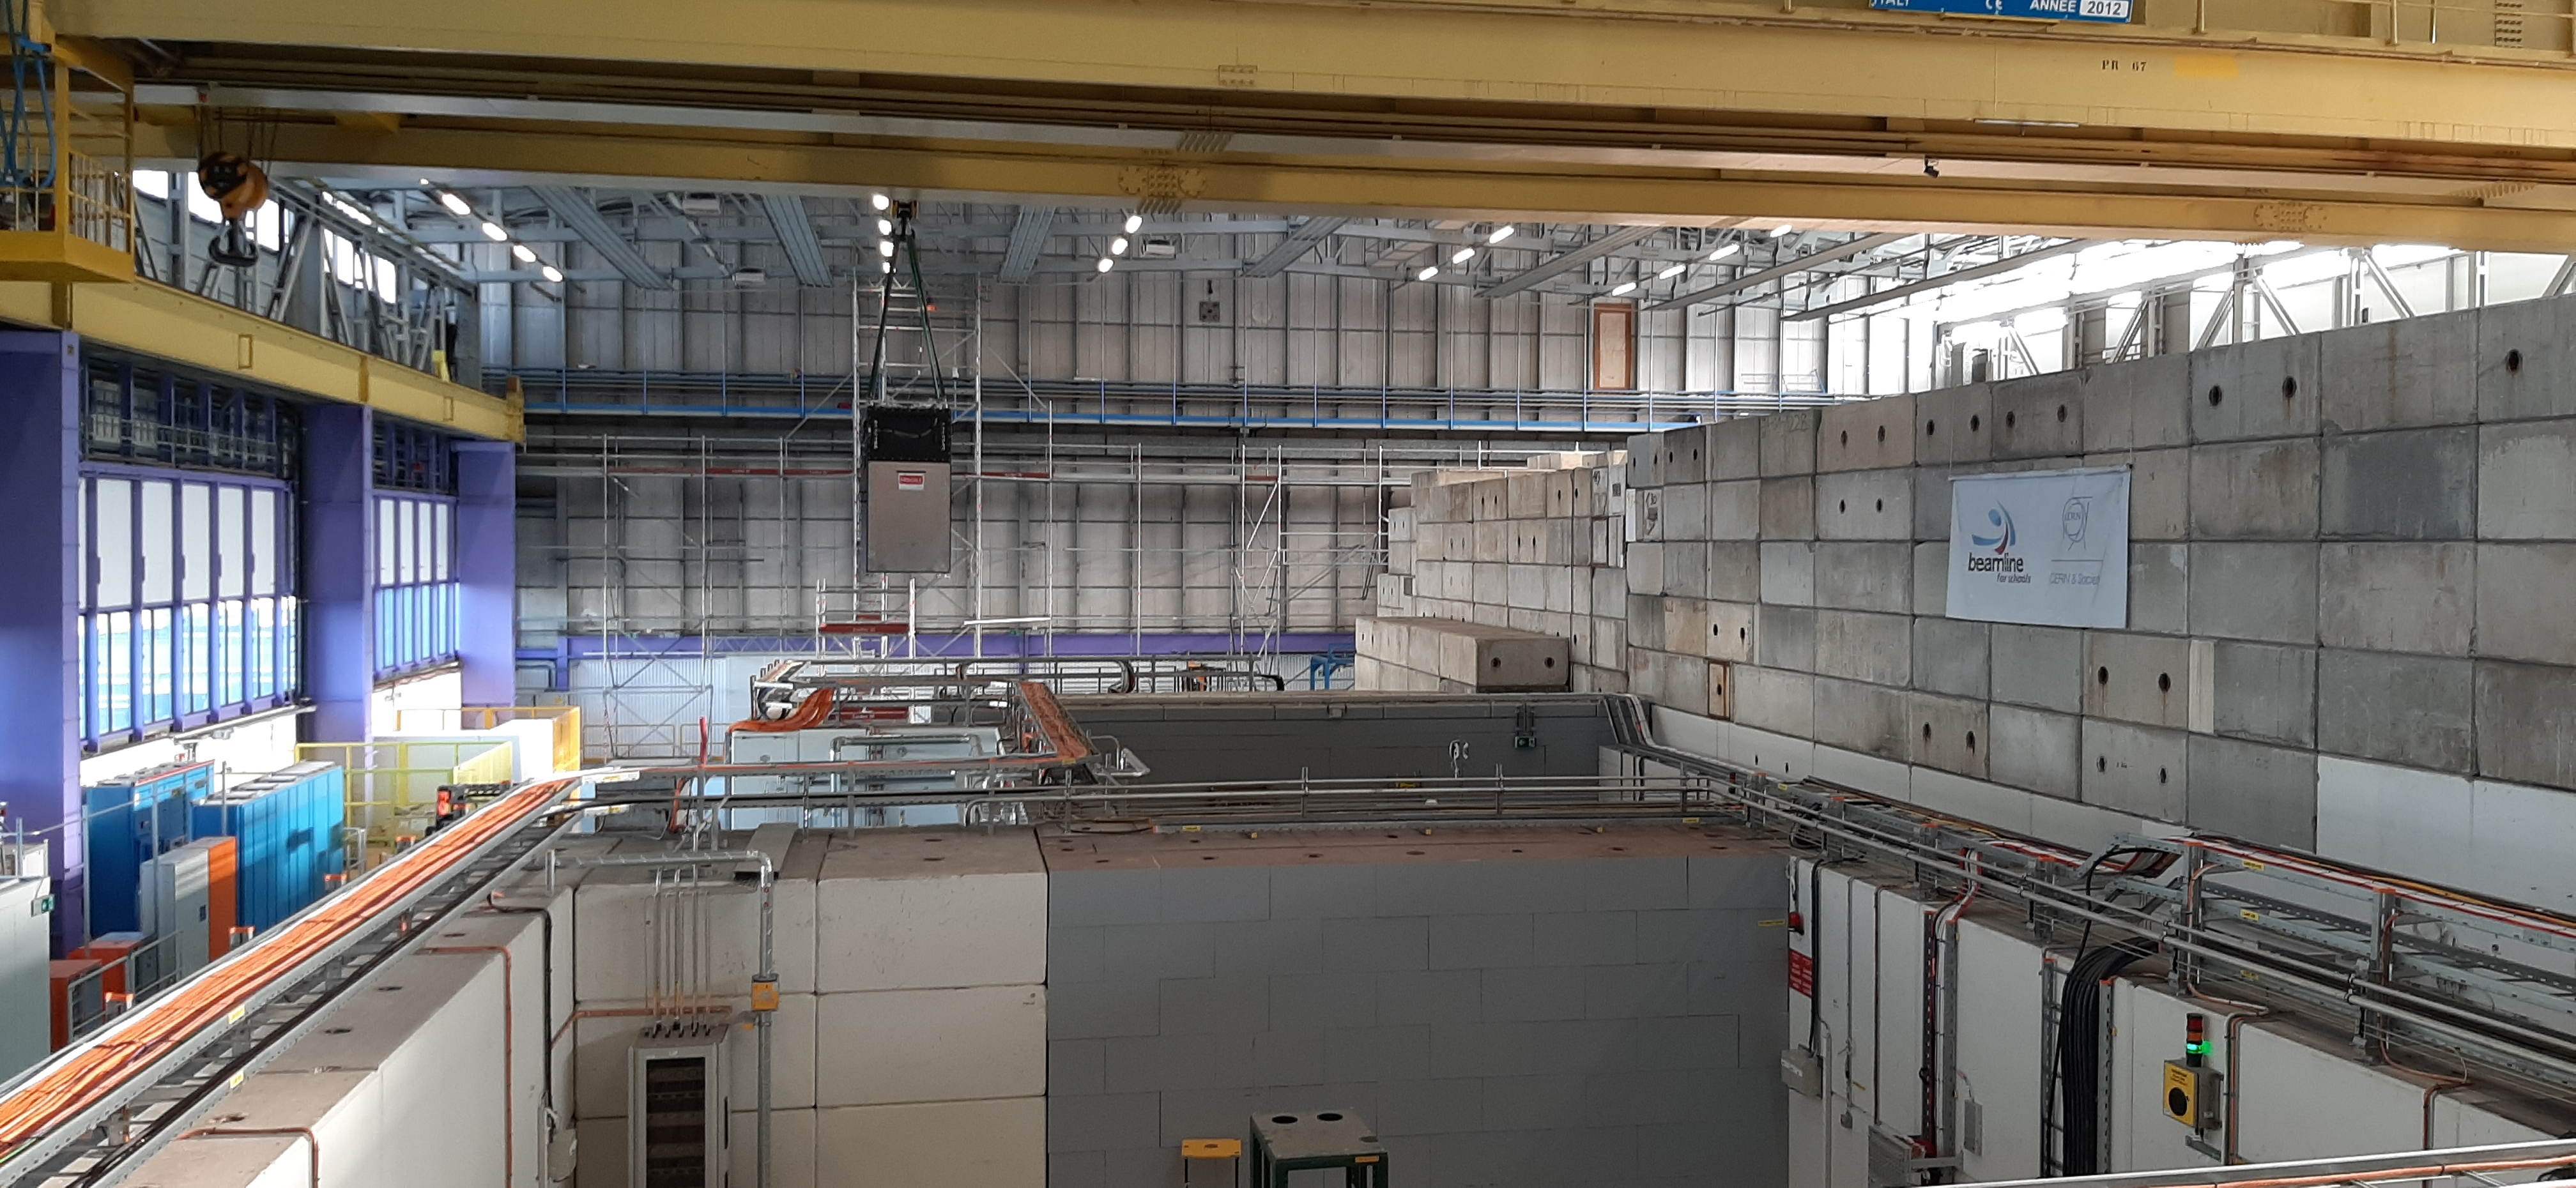
\includegraphics[width = 0.45\textwidth]{Plots/TORCH_transport_4.jpg}
    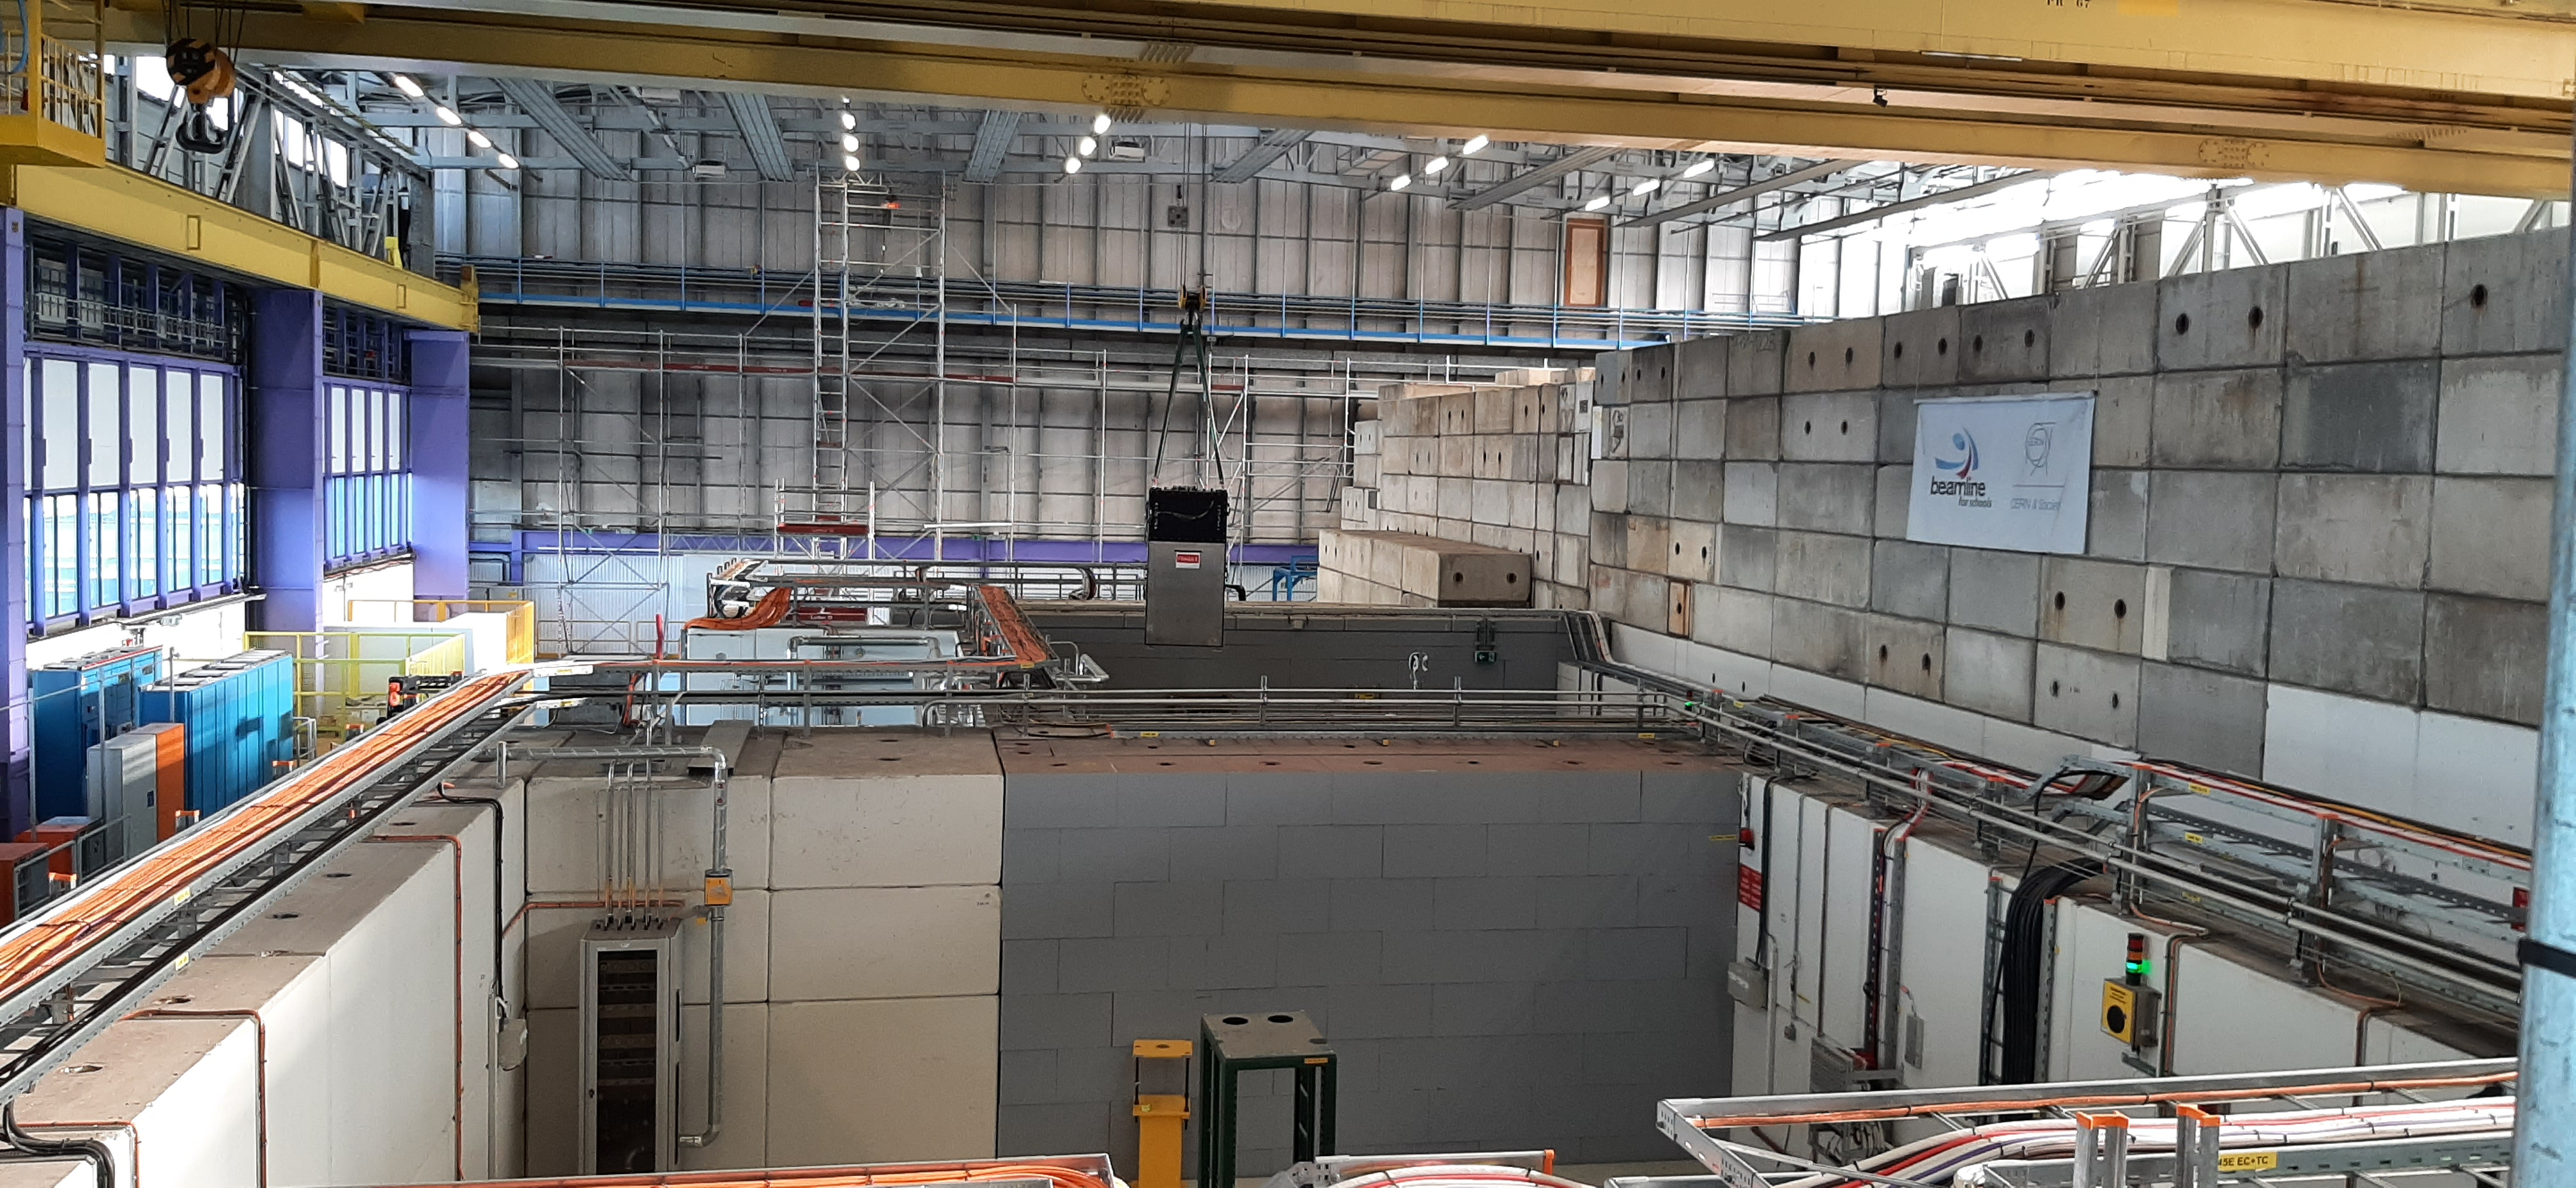
\includegraphics[width = 0.45\textwidth]{Plots/TORCH_transport_5.jpg}
    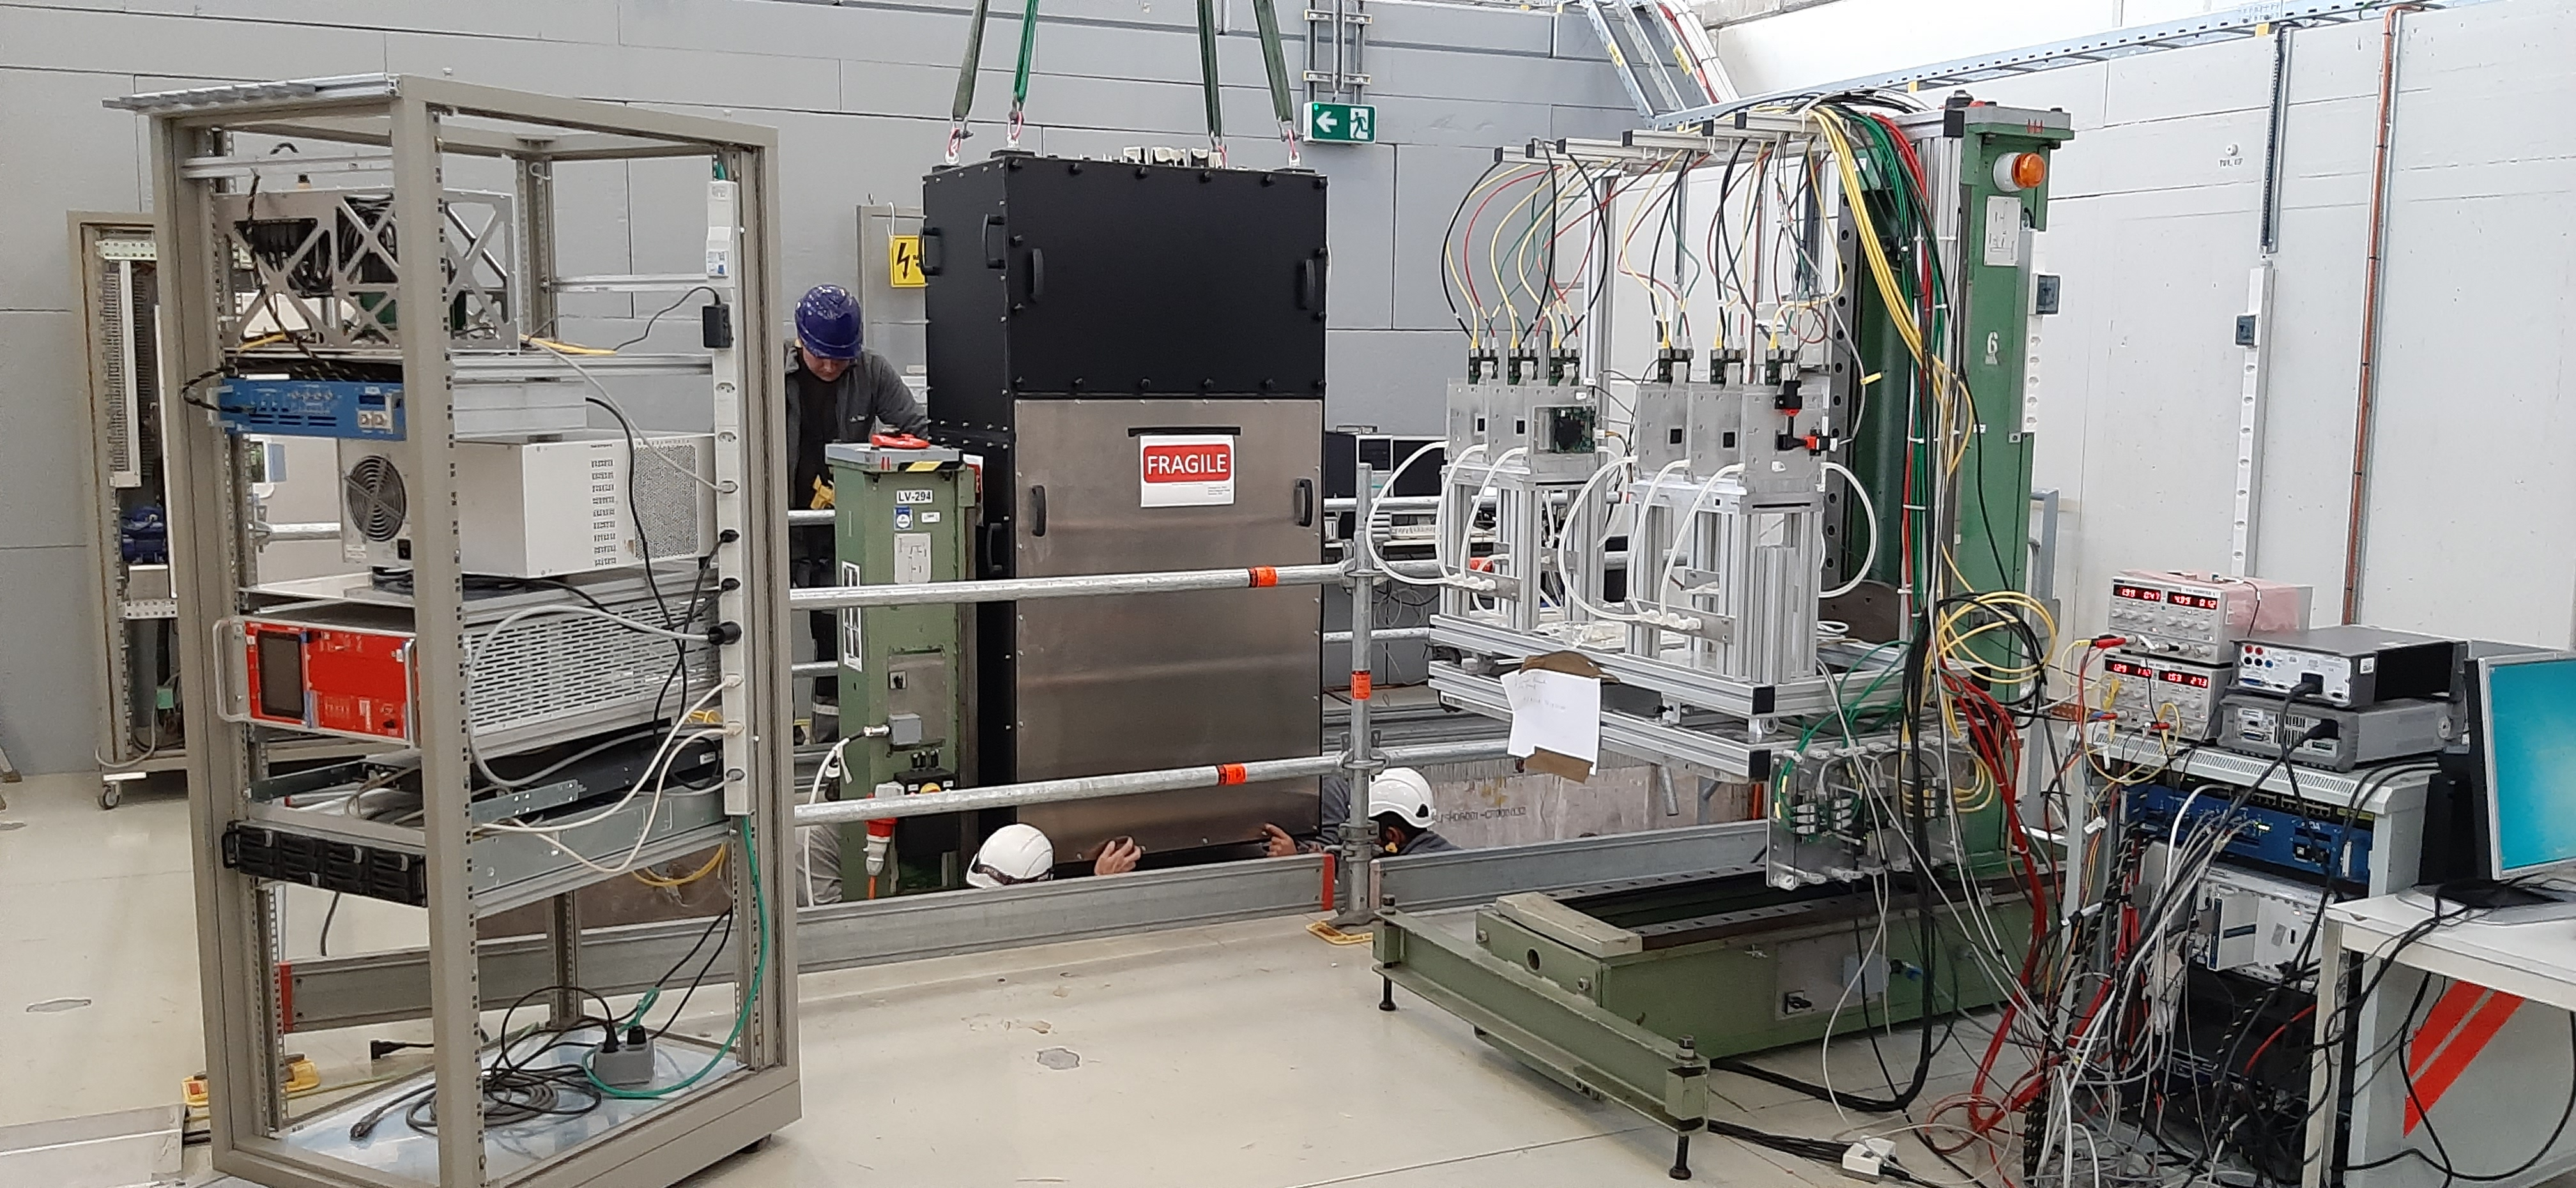
\includegraphics[width = 0.45\textwidth]{Plots/TORCH_transport_3.jpg}
  \end{figure}
\end{frame}

\begin{frame}{Get ready to turn everything on: Will it work?}
  \begin{center}
    \large We see light!
  \end{center}
  \begin{figure}
    \centering
    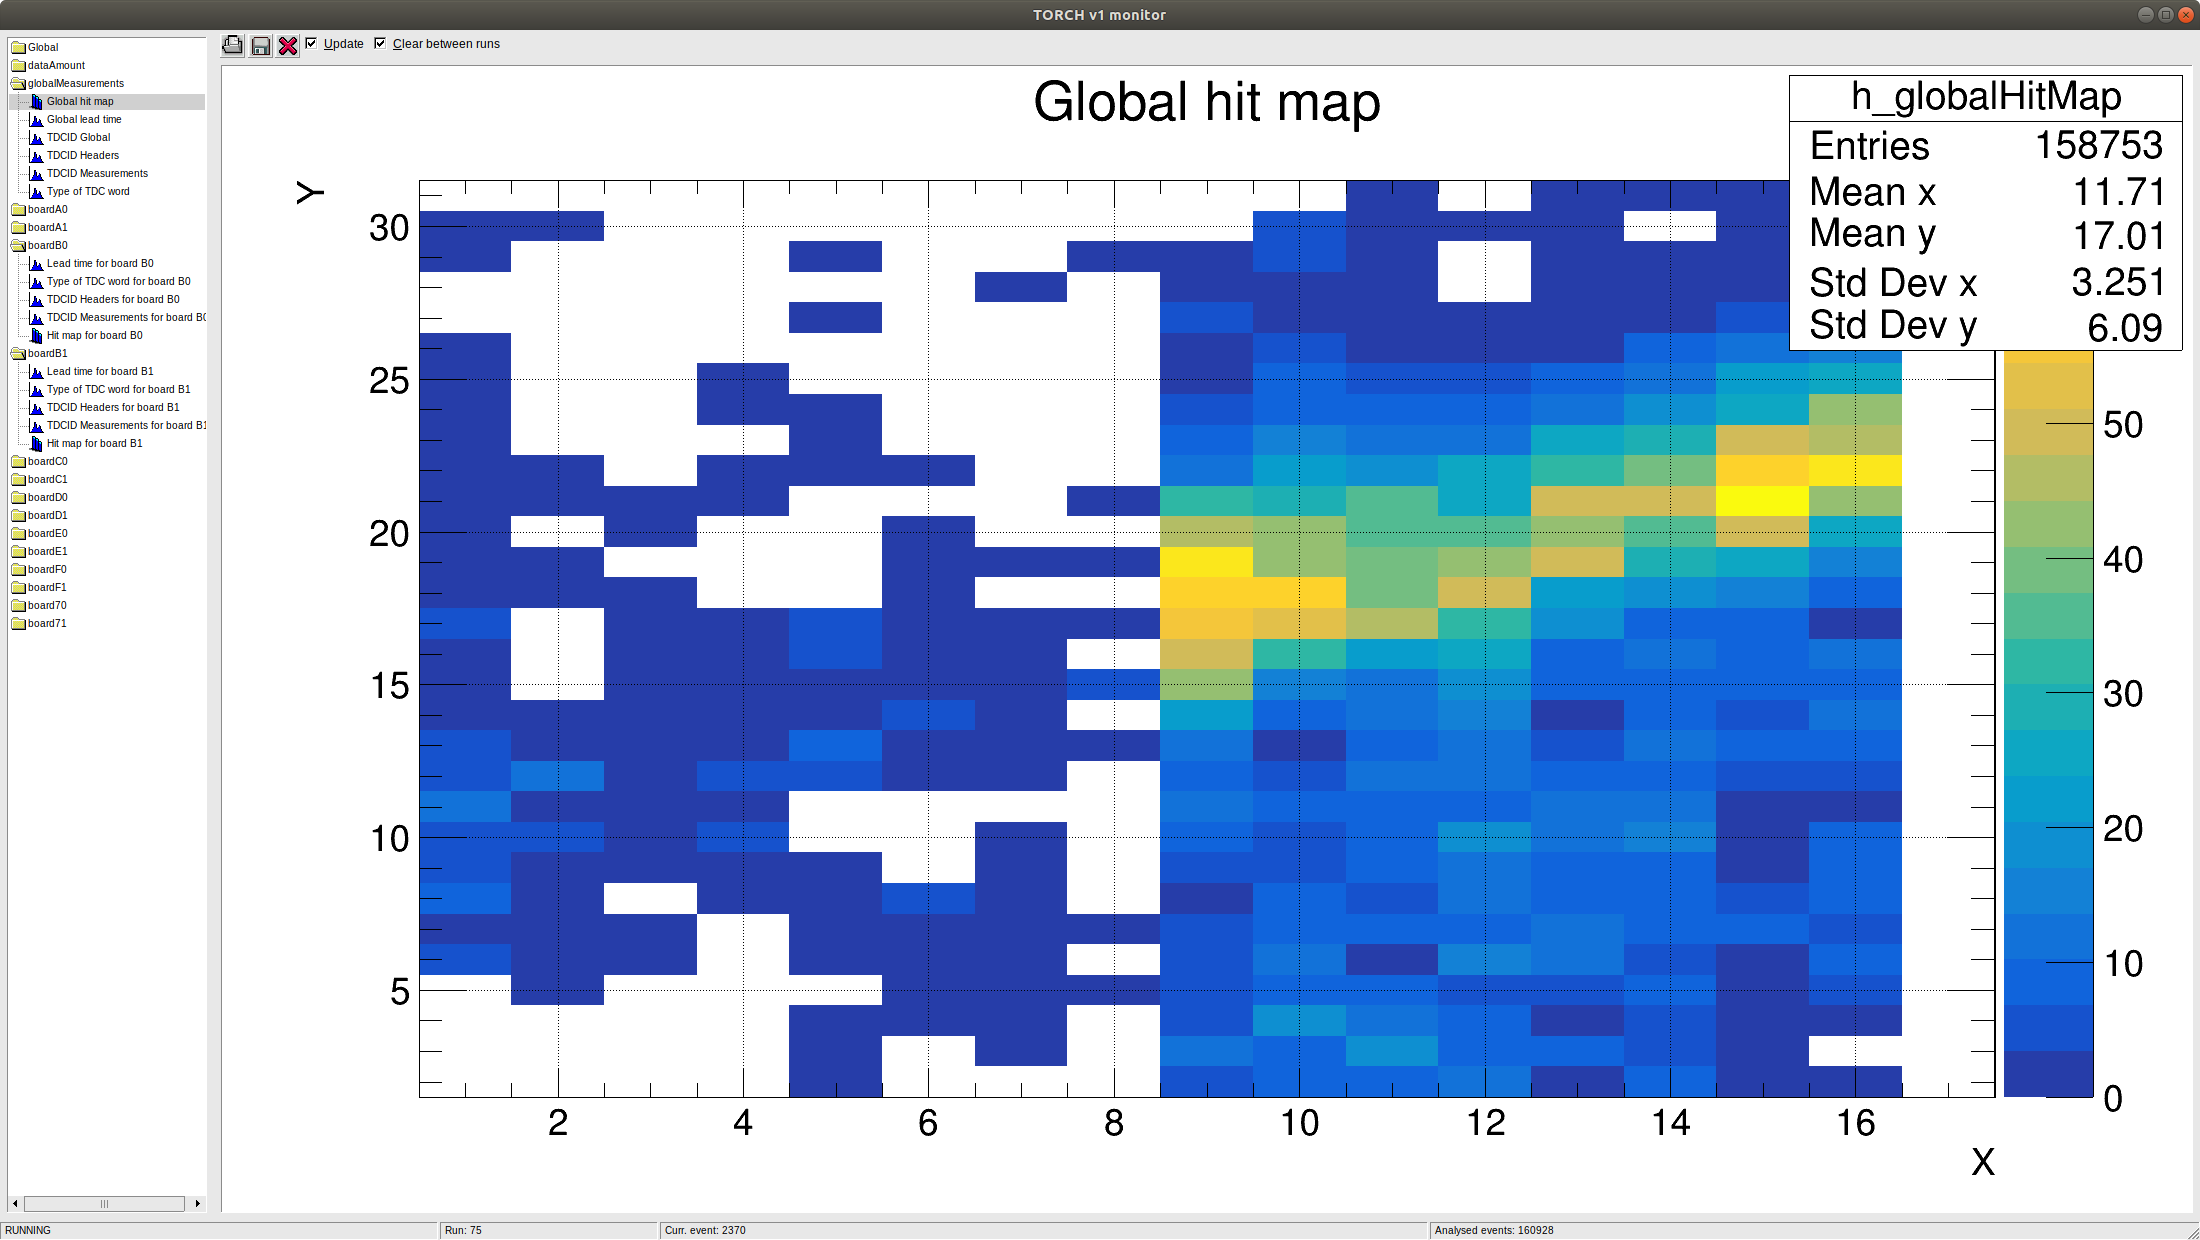
\includegraphics[width = 0.65\textwidth]{Plots/FirstHitMap.png}
  \end{figure}
  \vspace{-0.2cm}
  \begin{block}{Logbook entry 107}
    \textbf{First global hitmap}\\
    Global hitmap with MCP A and B, we can clearly see a band!
  \end{block}
\end{frame}

\begin{frame}{Get ready to turn everything on: Will it work?}
  \begin{center}
    \large But things weren't always running smoothly...
  \end{center}
  \begin{figure}
    \centering
    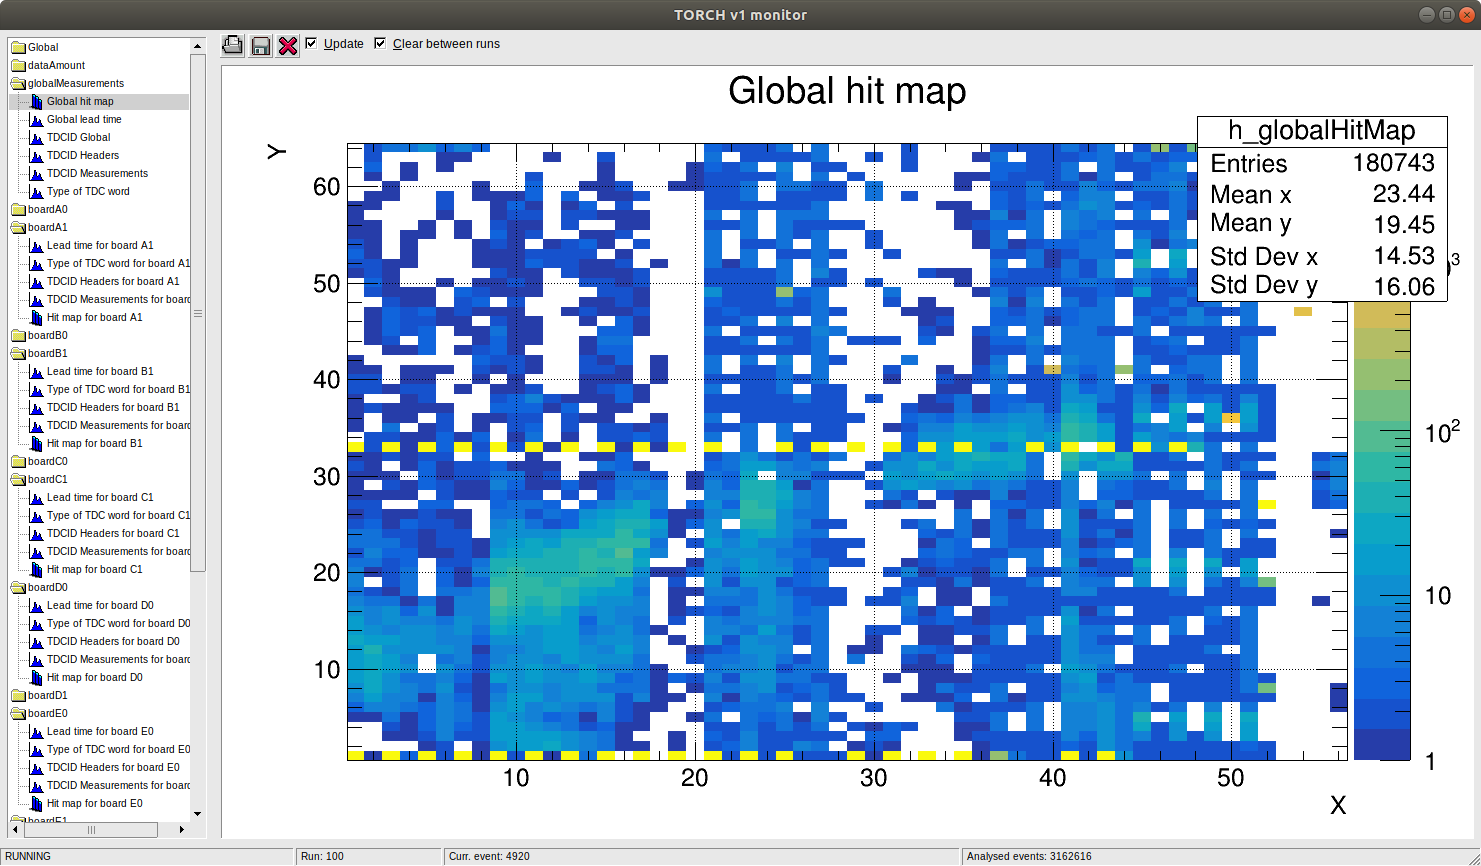
\includegraphics[width = 0.65\textwidth]{Plots/SaturdayGlobalHitMap.png}
  \end{figure}
  \vspace{-0.2cm}
  \begin{block}{Logbook entry 113}
    \textbf{Global hit map today}\\
    We've got a partially good global hit map after 3 hours of power cycling
  \end{block}
\end{frame}

\begin{frame}{Get ready to turn everything on: Will it work?}
  \begin{center}
    \large ... but we were always optimistic and together we found a solution!
  \end{center}
  \begin{block}{Logbook entry 130}
    \textbf{Run 163}\\
    Today we managed to get the MCPs powered up and in a stable condition in less than 1 hour!
  \end{block}
  \begin{center}
    From our experience, to ensure stable running we must:
  \end{center}
  \begin{enumerate}
    \item{Follow Marion's MCP startup procedure (logbook entry 125)}
    \item{Custom NINO thresholds (logbook entry 140)}
    \item{Increase HV on MCP C, D, E, F (logbook entry 141)}
  \end{enumerate}
\end{frame}

\begin{frame}{Get ready to turn everything on: Will it work?}
  \begin{figure}
    \centering
    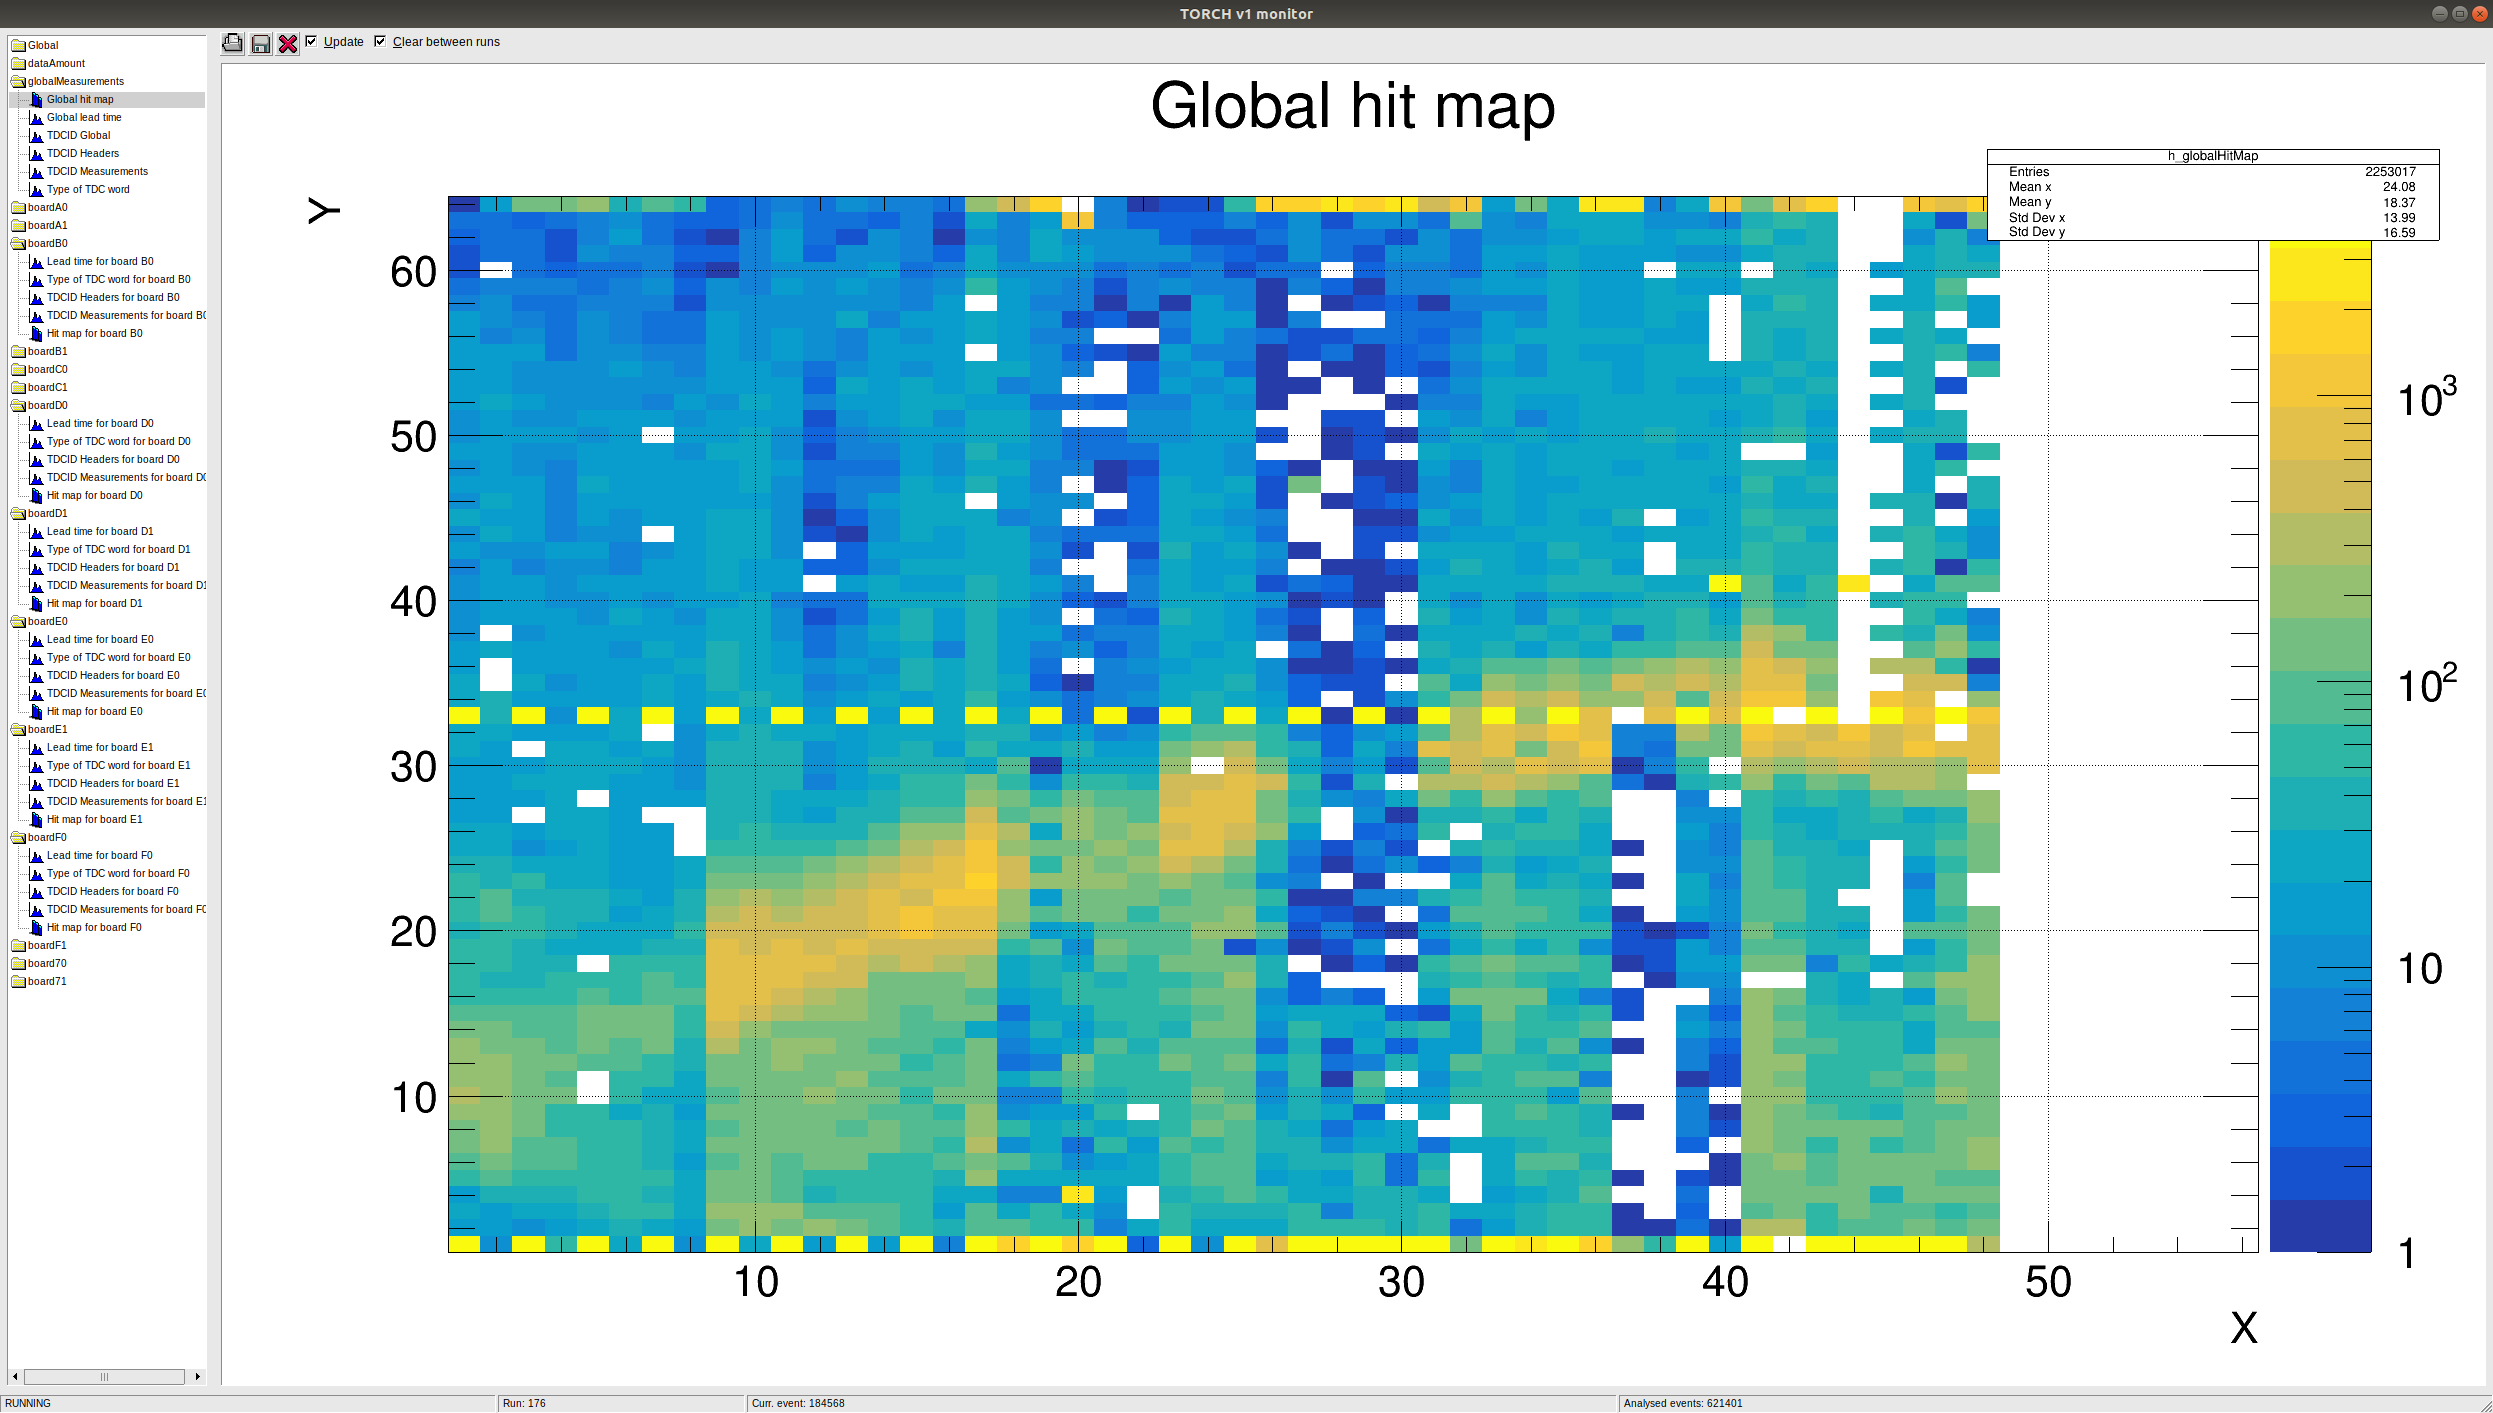
\includegraphics[width = 0.65\textwidth]{Plots/Run176HitMap.png}
  \end{figure}
  \vspace{-0.2cm}
  \begin{block}{Logbook entry 143}
    \textbf{Run 176}\\
    This run contains mostly good data ...
  \end{block}
\end{frame}

\begin{frame}{Get ready to turn everything on: Will it work?}
  \begin{center}
    However, not everything went smoothly and we had to accept that we cannot always have what we want
  \end{center}
  \begin{block}{Logbook entry 139}
    \textbf{Summary of MCPs}\\
    --We don't use MCP 7\\
    --MCP D have a huge deficit in the middle, this agrees with measurements from the lab\\
    --E1 is missing time references and but we see TORCH photons\\
    --F1 has some NINO threshold issues and we've tried to set these many times without any improvement
  \end{block}
\end{frame}

\section{Let's collect data: Beam positions}
\begin{frame}{Let's collect data: Beam positions}
  \begin{columns}
    \begin{column}{0.55\textwidth}
      \begin{itemize}
        \item{Week 3+4: Collect data!}
        \begin{itemize}
          \item{Huge dataset!}
          \item{New positions: 8, 9, 10, 11, 12}
          \item{Position 1 for comparison with previous test beam}
          \item{24/7 operation for 2 weeks}
          \item{INL runs at $\SI{8}{\giga\eV}$, with 100 million events per position}
        \end{itemize}
      \end{itemize}
    \end{column}
    \begin{column}{0.45\textwidth}
      \begin{figure}
        \centering
        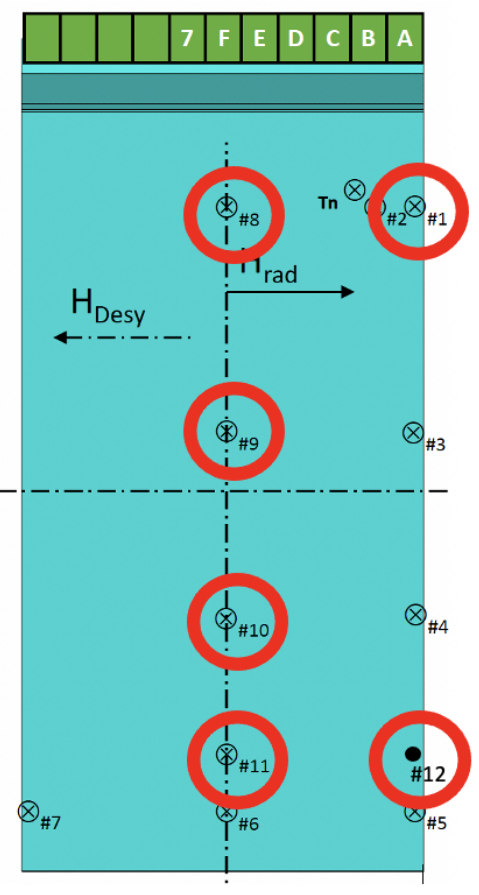
\includegraphics[width = 0.65\textwidth]{Plots/BeamPositions.png}
      \end{figure}
    \end{column}
  \end{columns}
\end{frame}

\section{Let's collect data: Beam momentum}
\begin{frame}{Let's collect data: Beam momentum}
  \begin{center}
    The regular runs contain data taken at $3$, $5$, $8$ and $\SI{10}{\giga\eV}$
  \end{center}
  \begin{figure}
    \centering
    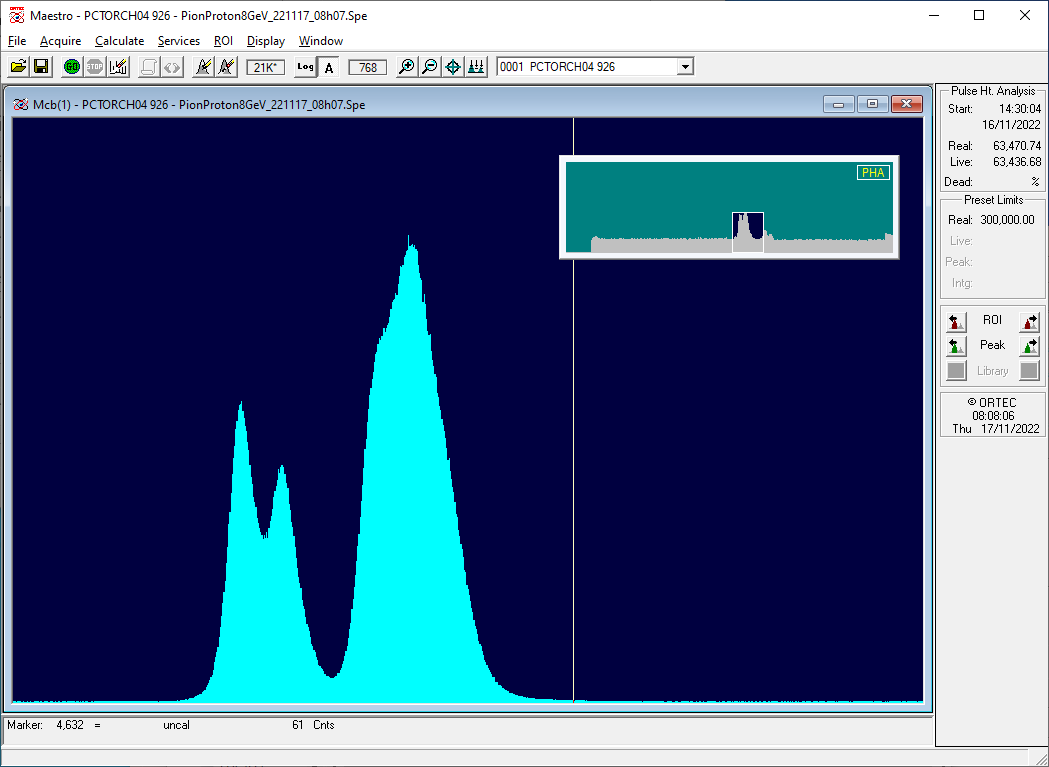
\includegraphics[width = 0.5\textwidth]{Plots/PionProton8GeV_221117_08h07.png}
  \end{figure}
  \begin{center}
    Beam momentum can be calibrated exactly using the ORTEC module
  \end{center}
\end{frame}

\section{Let's collect data: Number of events in regular runs}
\begin{frame}{Number of events in regular runs}
  \begin{center}
    \large Systematic data taking at each beam momentum and beam position
  \end{center}
  \vspace{0.4cm}
  \centering
  \footnotesize
  \begin{center}
    Number of events in regular runs
    \vspace{-0.3cm}
   \end{center}
  \begin{tabular}{|c|rrrr|}
    \hline
    \backslashbox{\#}{$p$} & $\SI{10}{\giga\eV}$ & $\SI{8}{\giga\eV}$ & $\SI{5}{\giga\eV}$ & $\SI{3}{\giga\eV}$ \\
    \hline
    1  & 882623  & 1283522 & 395017 & 62167 \\
    12 & 1086330 & 1054173 & 431413 & 56231 \\ 
    11 & 1706747 & 1018446 & 425828 & 57904 \\
    10 & 1071997 & 1012901 & 394197 & 70452 \\
    9  & 790394  & 1008021 & 412670 & 72505 \\
    8  & 1241379 & 1023918 & 402732 & 62167 \\
    \hline
  \end{tabular}
  \vspace{0.2cm}
  \begin{center}
    \large Around 1 million events at $8$ and $\SI{10}{\giga\eV}$, less at $3$ and $\SI{5}{\giga\eV}$
  \end{center}
\end{frame}

\section{Let's collect data: Number of events in special runs}
\begin{frame}{Number of events in special}
  \begin{center}
    \large We also had time for special runs at the end, with different beam momenta and Cherenkov pressures
  \end{center}
  \centering
  \footnotesize
  \begin{center}
    \large Number of events with different Cherenkov pressures
   \end{center}
  \begin{tabular}{|c|rrrrrr|}
    \hline
    \backslashbox{\#}{$p$} & $\SI{5}{\giga\eV}$ & $\SI{8}{\giga\eV}$ & $\SI{10}{\giga\eV}$ & $\SI{12}{\giga\eV}$ & $\SI{14}{\giga\eV}$ & $\SI{15}{\giga\eV}$ \\
    \hline
    8 & 155603 & 300402 & 466233  & 592427  & 536363  & 547406 \\
    9 & 181862 & 405189 & 1460513 & 1062475 & 1077304 & 575346 \\
    \hline
  \end{tabular}
  \begin{center}
    \vspace{0.5cm}
    Number of events with same Cherenkov pressures
    \vspace{-0.3cm}
   \end{center}
  \begin{tabular}{|c|rrrr|}
    \hline
    \backslashbox{\#}{$p$} & $\SI{3}{\giga\eV}$ & $\SI{5}{\giga\eV}$ & $\SI{8}{\giga\eV}$ & $\SI{10}{\giga\eV}$ \\
    \hline
    8 & 24654 & 116874 & 110861 & 126796 \\
    \hline
  \end{tabular}
\end{frame}

\section{Summary}
\begin{frame}{Summary}
  \begin{itemize}
    \setlength\itemsep{1.0em}
    \item{Week 1: Setup and installation went smoothly}
    \item{Week 2: We successfully stabilised the system}
    \item{Week 3+4: We collected the largest dataset that the TORCH collaboration has ever seen!}
    \item{More detailed talks by David, Rui, Stoyan, Christoph, Rok, Marion, Michal and Ivan}
  \end{itemize}
  \begin{center}
    \huge Thank you all for a successful test beam!
  \end{center}
  \begin{block}{More wise words}
    \textit{``Teamwork divides the task and doubles the success''}\\~\quad\quad-- The Internet
  \end{block}
\end{frame}

\section{Backup: Database of runs}
\begin{frame}[fragile]{Backup: Database of runs}
  \begin{itemize}
    \setlength\itemsep{0.5em}
    \item{I also tried to make an overview of all runs}
    \item{No way to make it readable or useful...}
    \item{Solution: I put the whole spread sheet into a pandas dataframe!}
    \item{Available on EOS: \texttt{\tiny/eos/experiment/torch/data/BeamTests\_Data/2022/PS\_T9/TORCH\_runs.pickle}}
    \item{Instructions for loading dataframe:}
  \end{itemize}
  \vspace{0.3cm}
  \begin{lstlisting}[language=bash]
    $   lb-conda default/2022-12-06 python
    >>> import pandas as pd
    >>> df = pd.read_pickle('TORCH_runs.pickle')
  \end{lstlisting}
\end{frame}

\begin{frame}[fragile]{Backup: Database of runs}
  \vspace{0.3cm}
  \tiny
  \begin{lstlisting}[language=bash]
    >>> df[25:30]
        Run  p Position Events    INL  Special  HighPr  LowPr          Comment
    25  265  8       12  95176  False    False     NaN    NaN  MIMOSA0 missing
    26  267  8       12  38516  False    False     NaN    NaN  MIMOSA0 missing
    27  268  8       12  21142  False    False     NaN    NaN                 
    28  270  8       12  89594  False    False     NaN    NaN                 
    29  271  8       12   3312  False    False     NaN    NaN
  \end{lstlisting}
  \vspace{0.2cm}
  \begin{lstlisting}[language=bash]
    >>> df[(df['INL'] == True) & (df['Position'] == 9)]
        Run  p Position Events   INL  Special  HighPr  LowPr Comment
    58  363  8        9    NaN  True    False     NaN    NaN        
    59  364  8        9    NaN  True    False     NaN    NaN        
    60  365  8        9    NaN  True    False     NaN    NaN        
    65  374  8        9    NaN  True    False     NaN    NaN
  \end{lstlisting}
  \vspace{0.2cm}
  \begin{lstlisting}[language=bash]
    >>> df[(df['Special'] == True) & (df['p'] == 8)]
         Run  p Position  Events    INL  Special  HighPr  LowPr Comment
    157  586  8        9  236853  False     True     9.0    2.0        
    158  588  8        9  168336  False     True     9.0    2.0        
    178  625  8        8  300402  False     True     9.0    2.0        
    188  635  8        8  100246  False     True     2.0    2.0        
    189  636  8        8   10615  False     True     2.0    2.0
  \end{lstlisting}
\end{frame}

\end{document}